% k-resultados.tex
% !TEX root = z-main.tex

\section{Resultados}

% En esta sección se presentan los modelos tridimensionales de los montículos analizados.
% Cada subsección incluye el panel de vistas generado (malla, sólido y texturizado).


\FloatBarrier
\subsection{Montículo 3}


\begin{figure}[!htbp]
    \centering
    \caption{Montículo 3, panel de vistas}
    \label{fig:m3-panel}
    % ----- Fila 1 -----
    \begin{subfigure}{0.48\textwidth}
        \centering
        \caption{Vista en malla (wireframe)}
        \label{fig:m3-wire}
        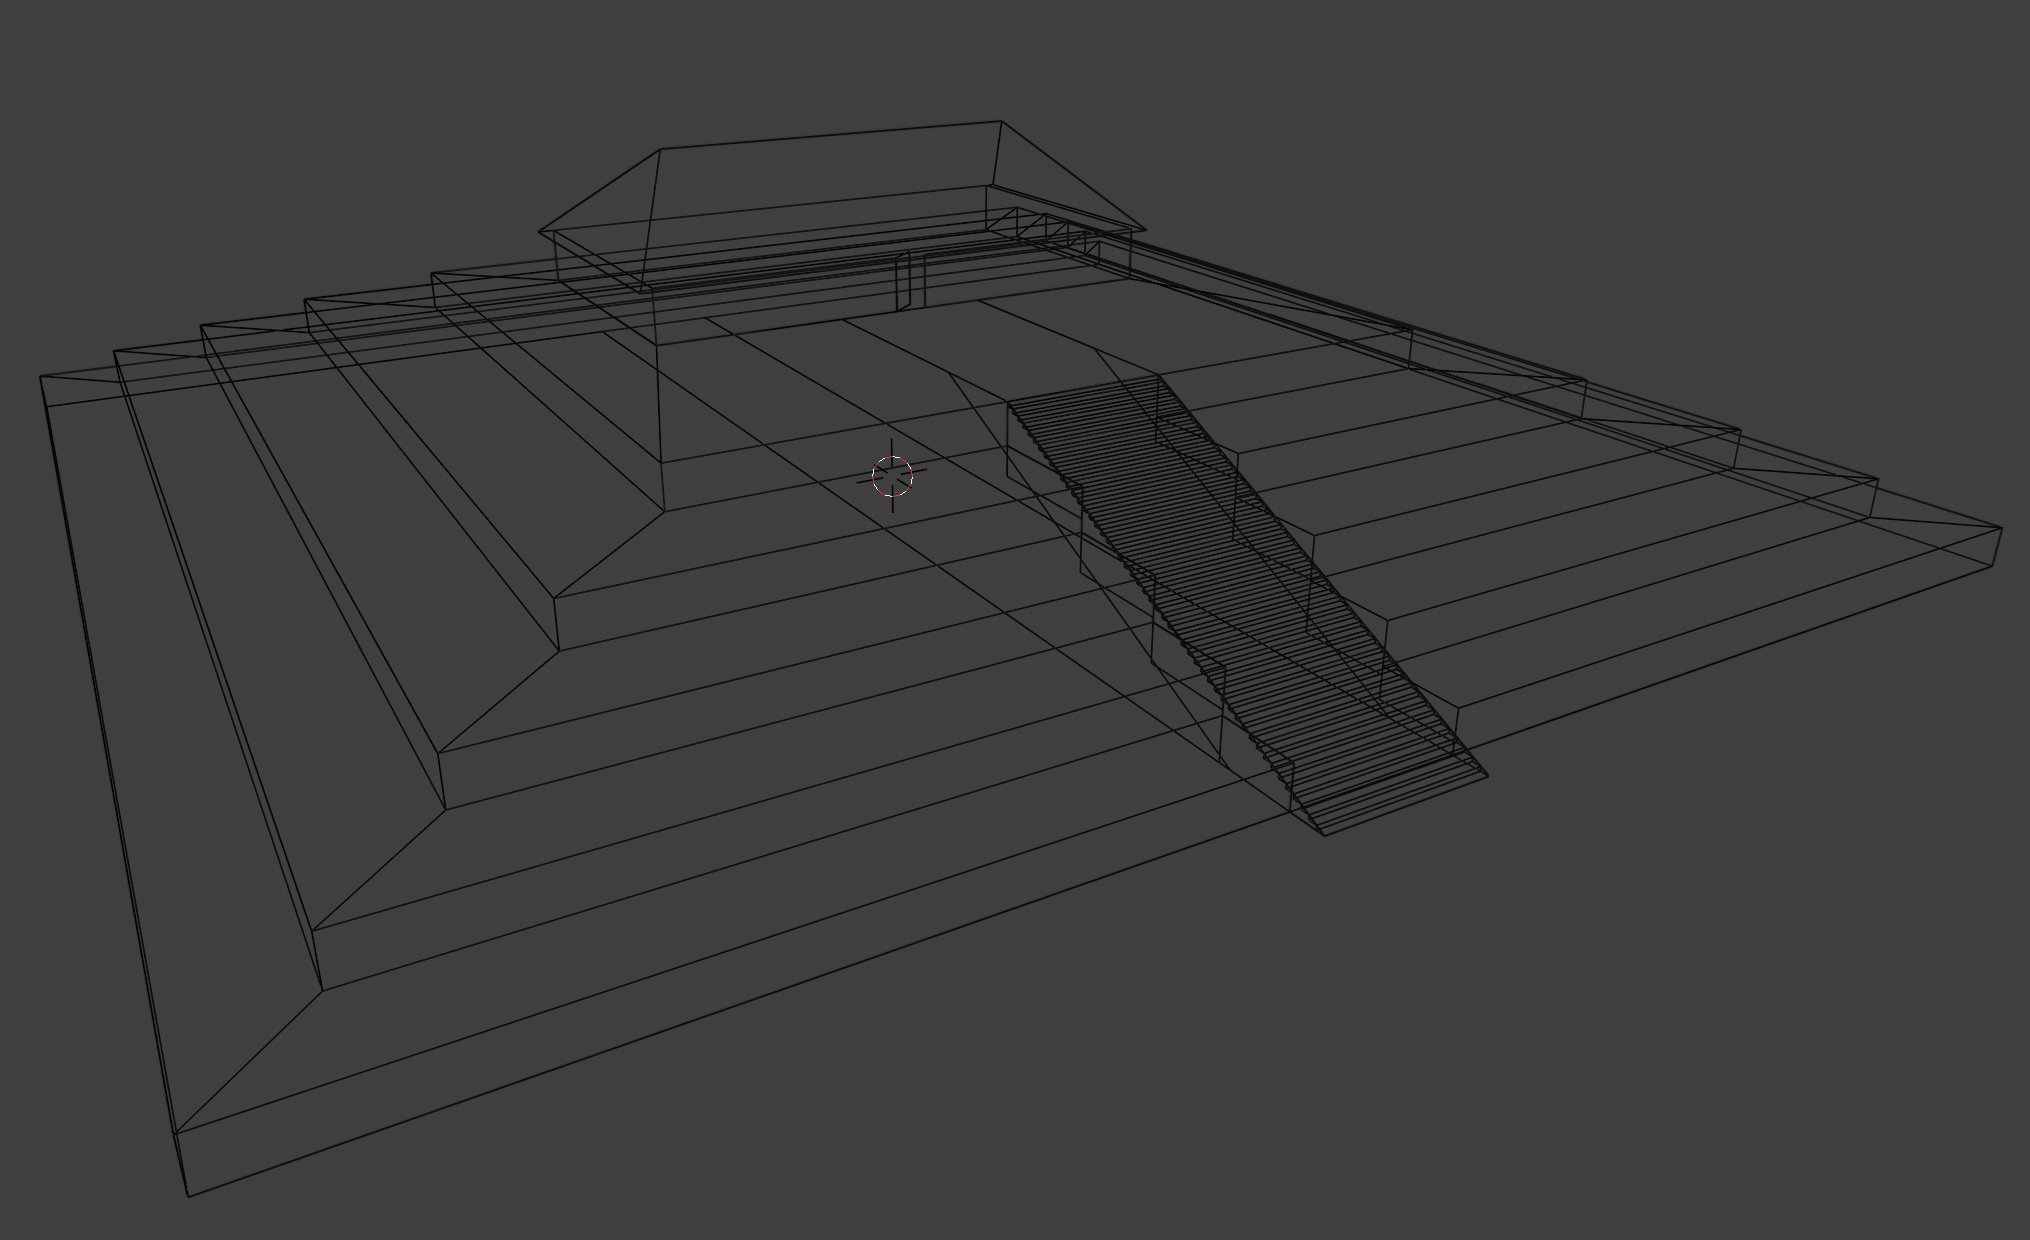
\includegraphics[width=\linewidth]{resultados/figures/m3/m3_wireframe.png}
    \end{subfigure}\hfill
    \begin{subfigure}{0.48\textwidth}
        \centering
        \caption{Vista sólida sin texturas}
        \label{fig:m3-solid}
        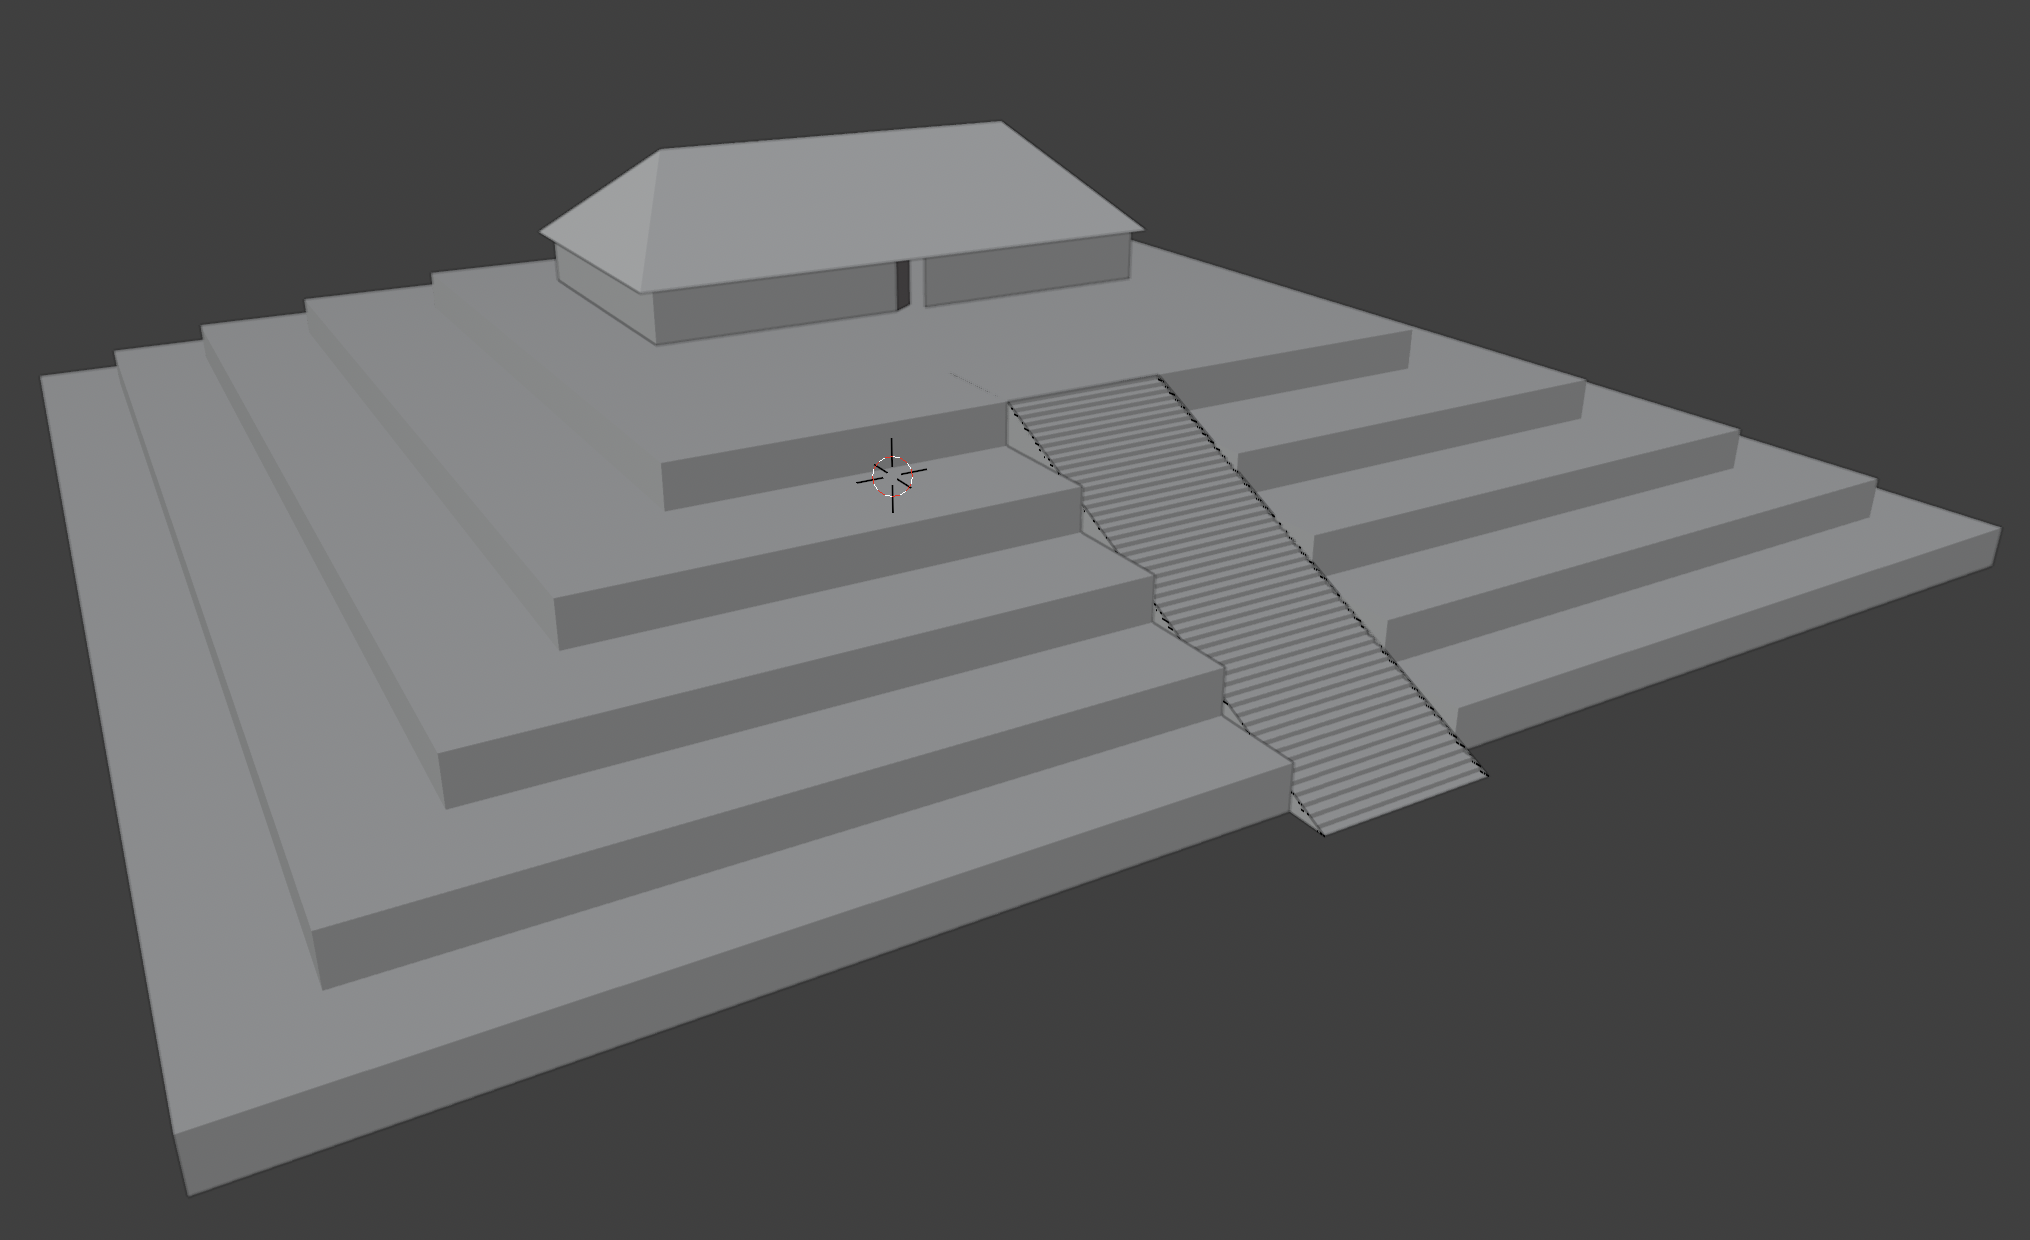
\includegraphics[width=\linewidth]{resultados/figures/m3/m3_solid.png}
    \end{subfigure}

    \vspace{0.6em}

    % ----- Fila 2 -----
    \begin{subfigure}{0.48\textwidth}
        \centering
        \caption{Vista con materiales/texturas}
        \label{fig:m3-textured}
        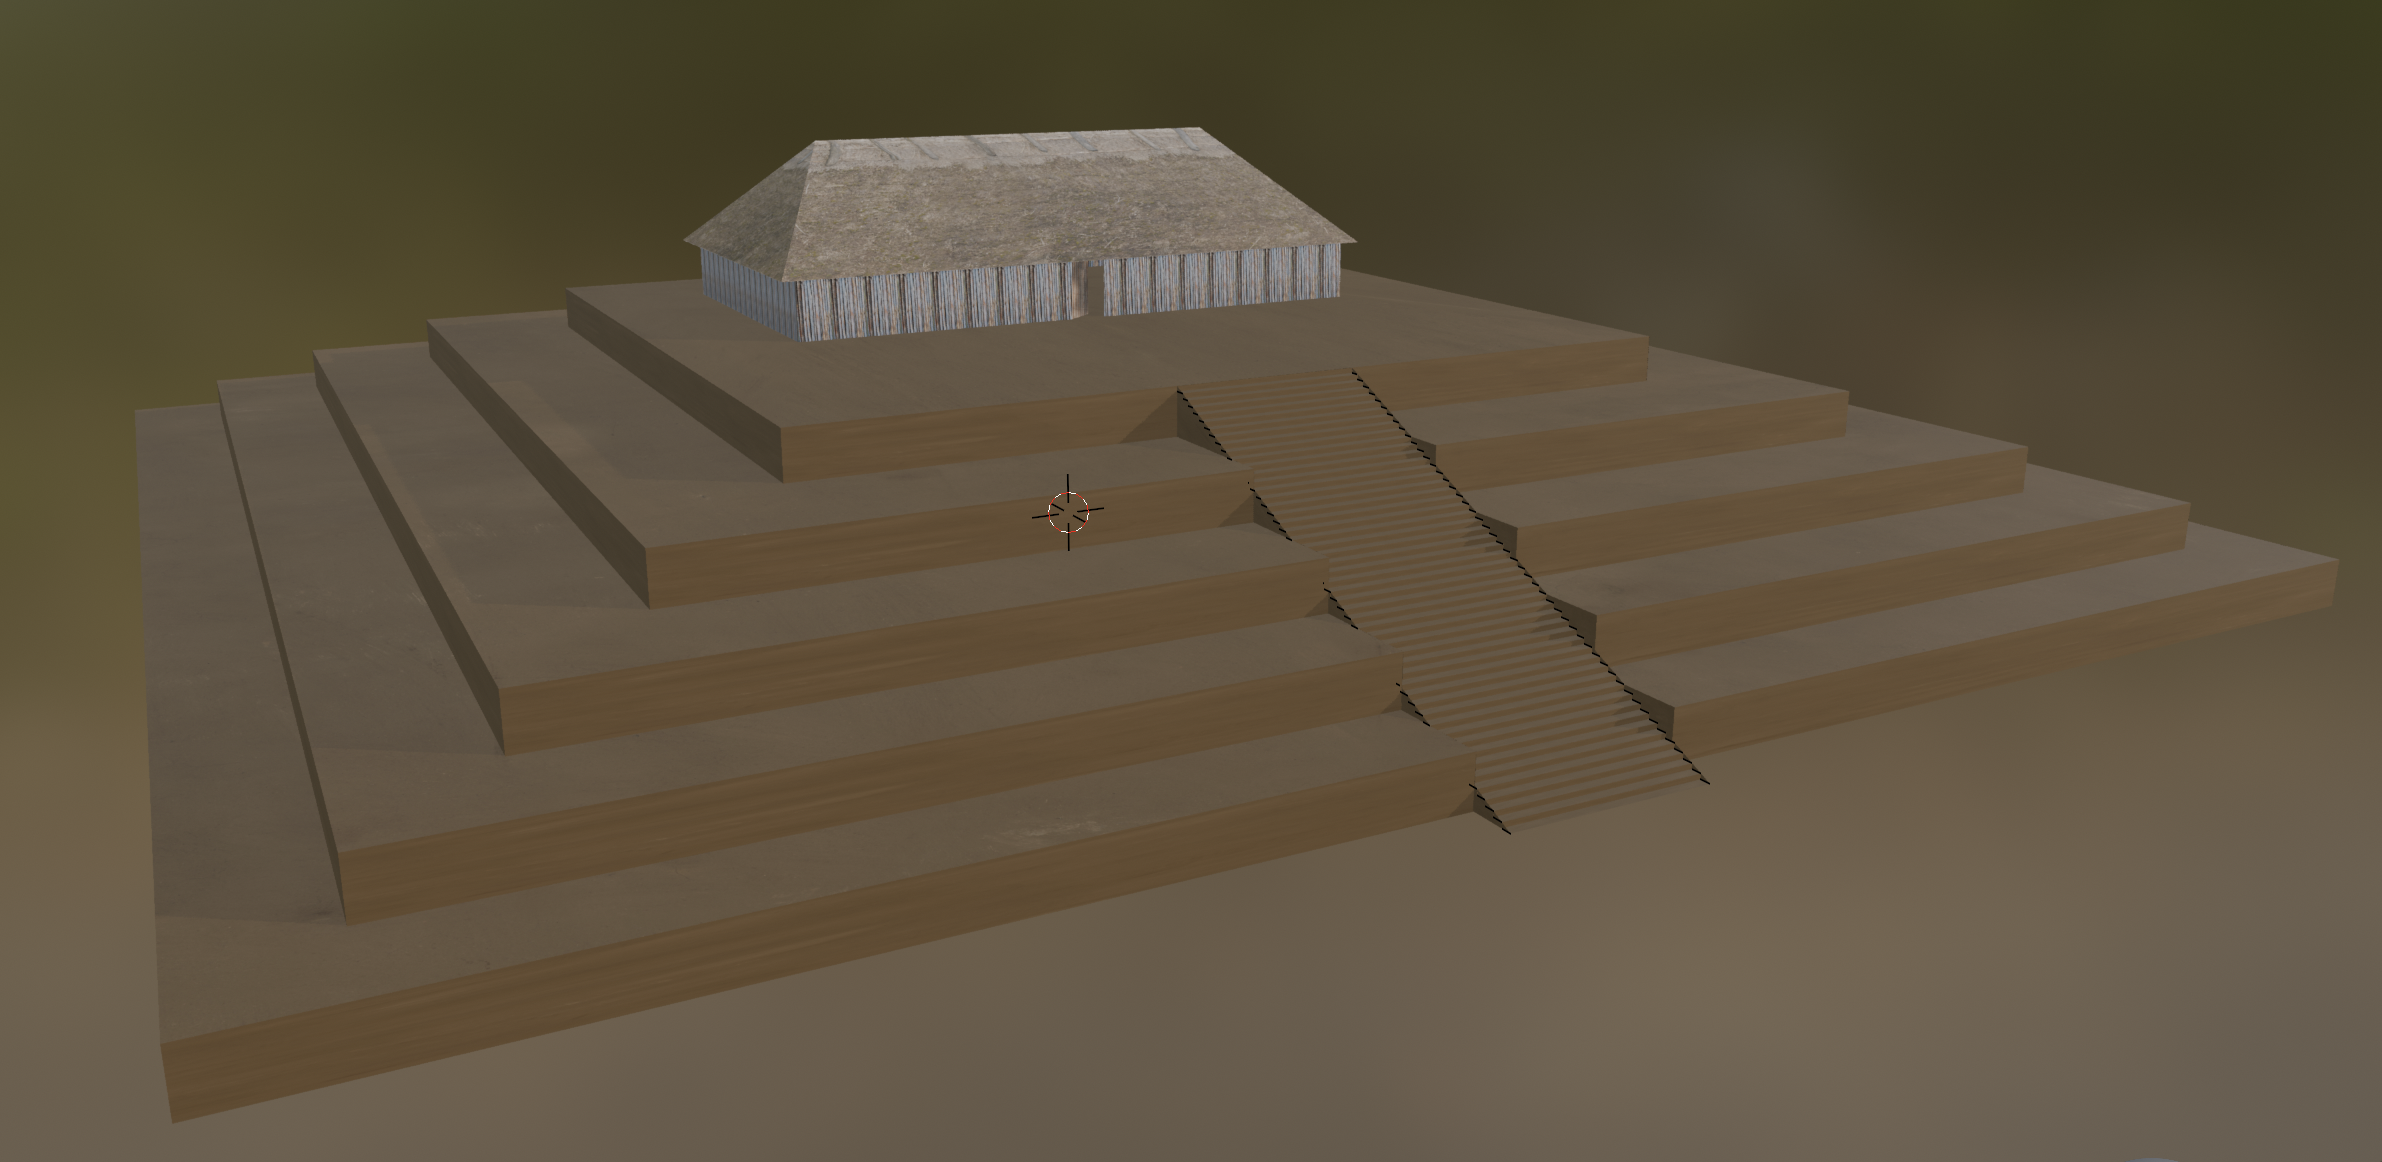
\includegraphics[width=\linewidth]{resultados/figures/m3/m3_textured_viewport.png}
    \end{subfigure}
\end{figure}
\FloatBarrier

\begin{figure}[!htbp]
    \centering
    \caption{Montículo 3 visualizado en la aplicación de realidad aumentada, mostrando la reconstrucción superpuesta en el entorno real del parque arqueológico}
    \label{fig:m3-ar}
    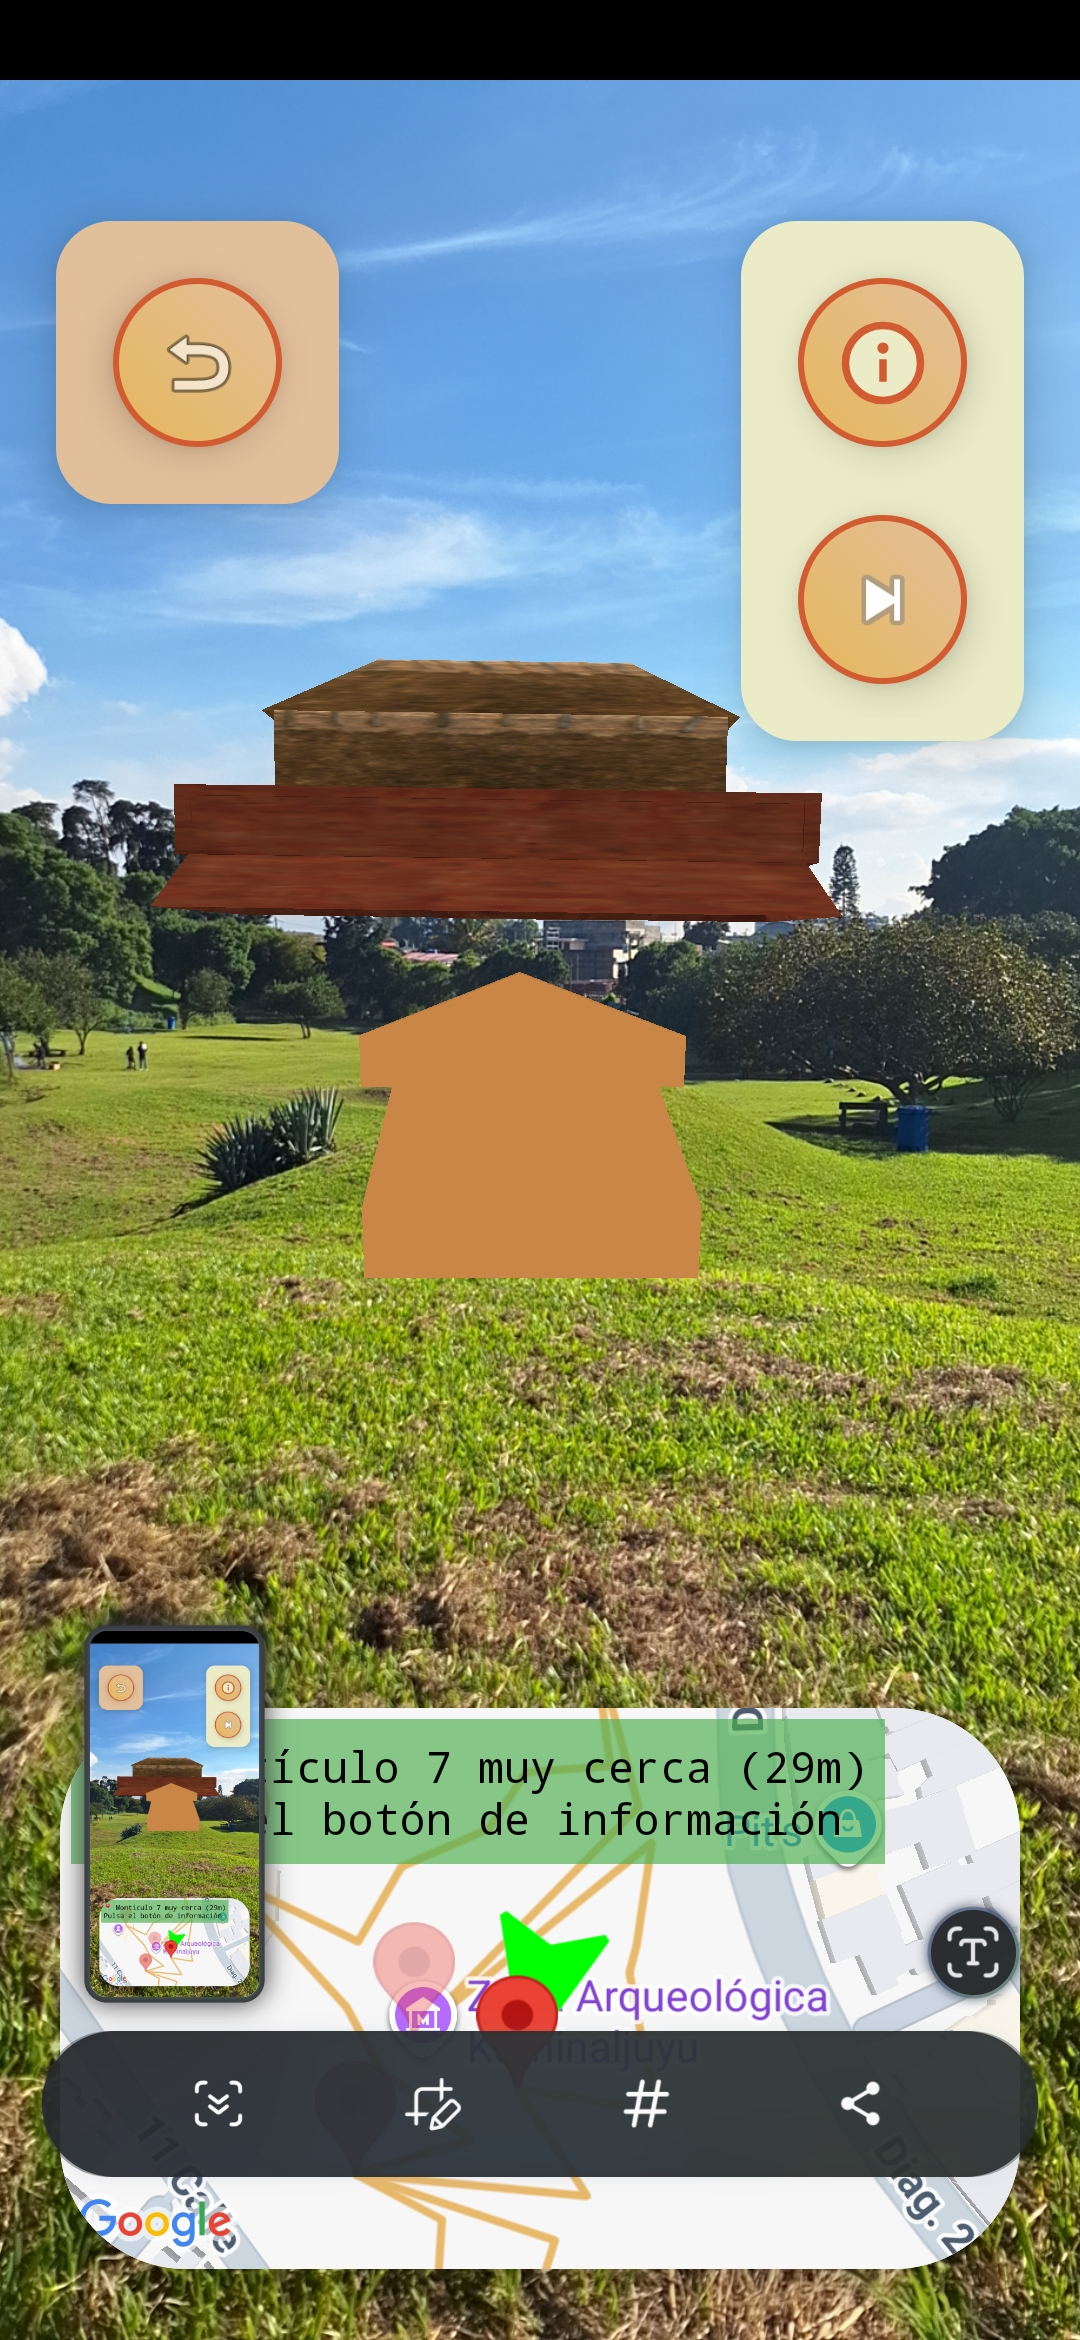
\includegraphics[width=0.48\linewidth]{resultados/figures/m3/m3_ar.jpg}
\end{figure}
\clearpage
\FloatBarrier
\subsection{Montículo 7}

\begin{figure}[!htbp]
    \centering
    \caption{Montículo 7, panel de vistas}
    \label{fig:m7-panel}
    % ----- Fila 1 -----
    \begin{subfigure}{0.48\textwidth}
        \centering
        \caption{Vista en malla (wireframe)}
        \label{fig:m7-wire}
        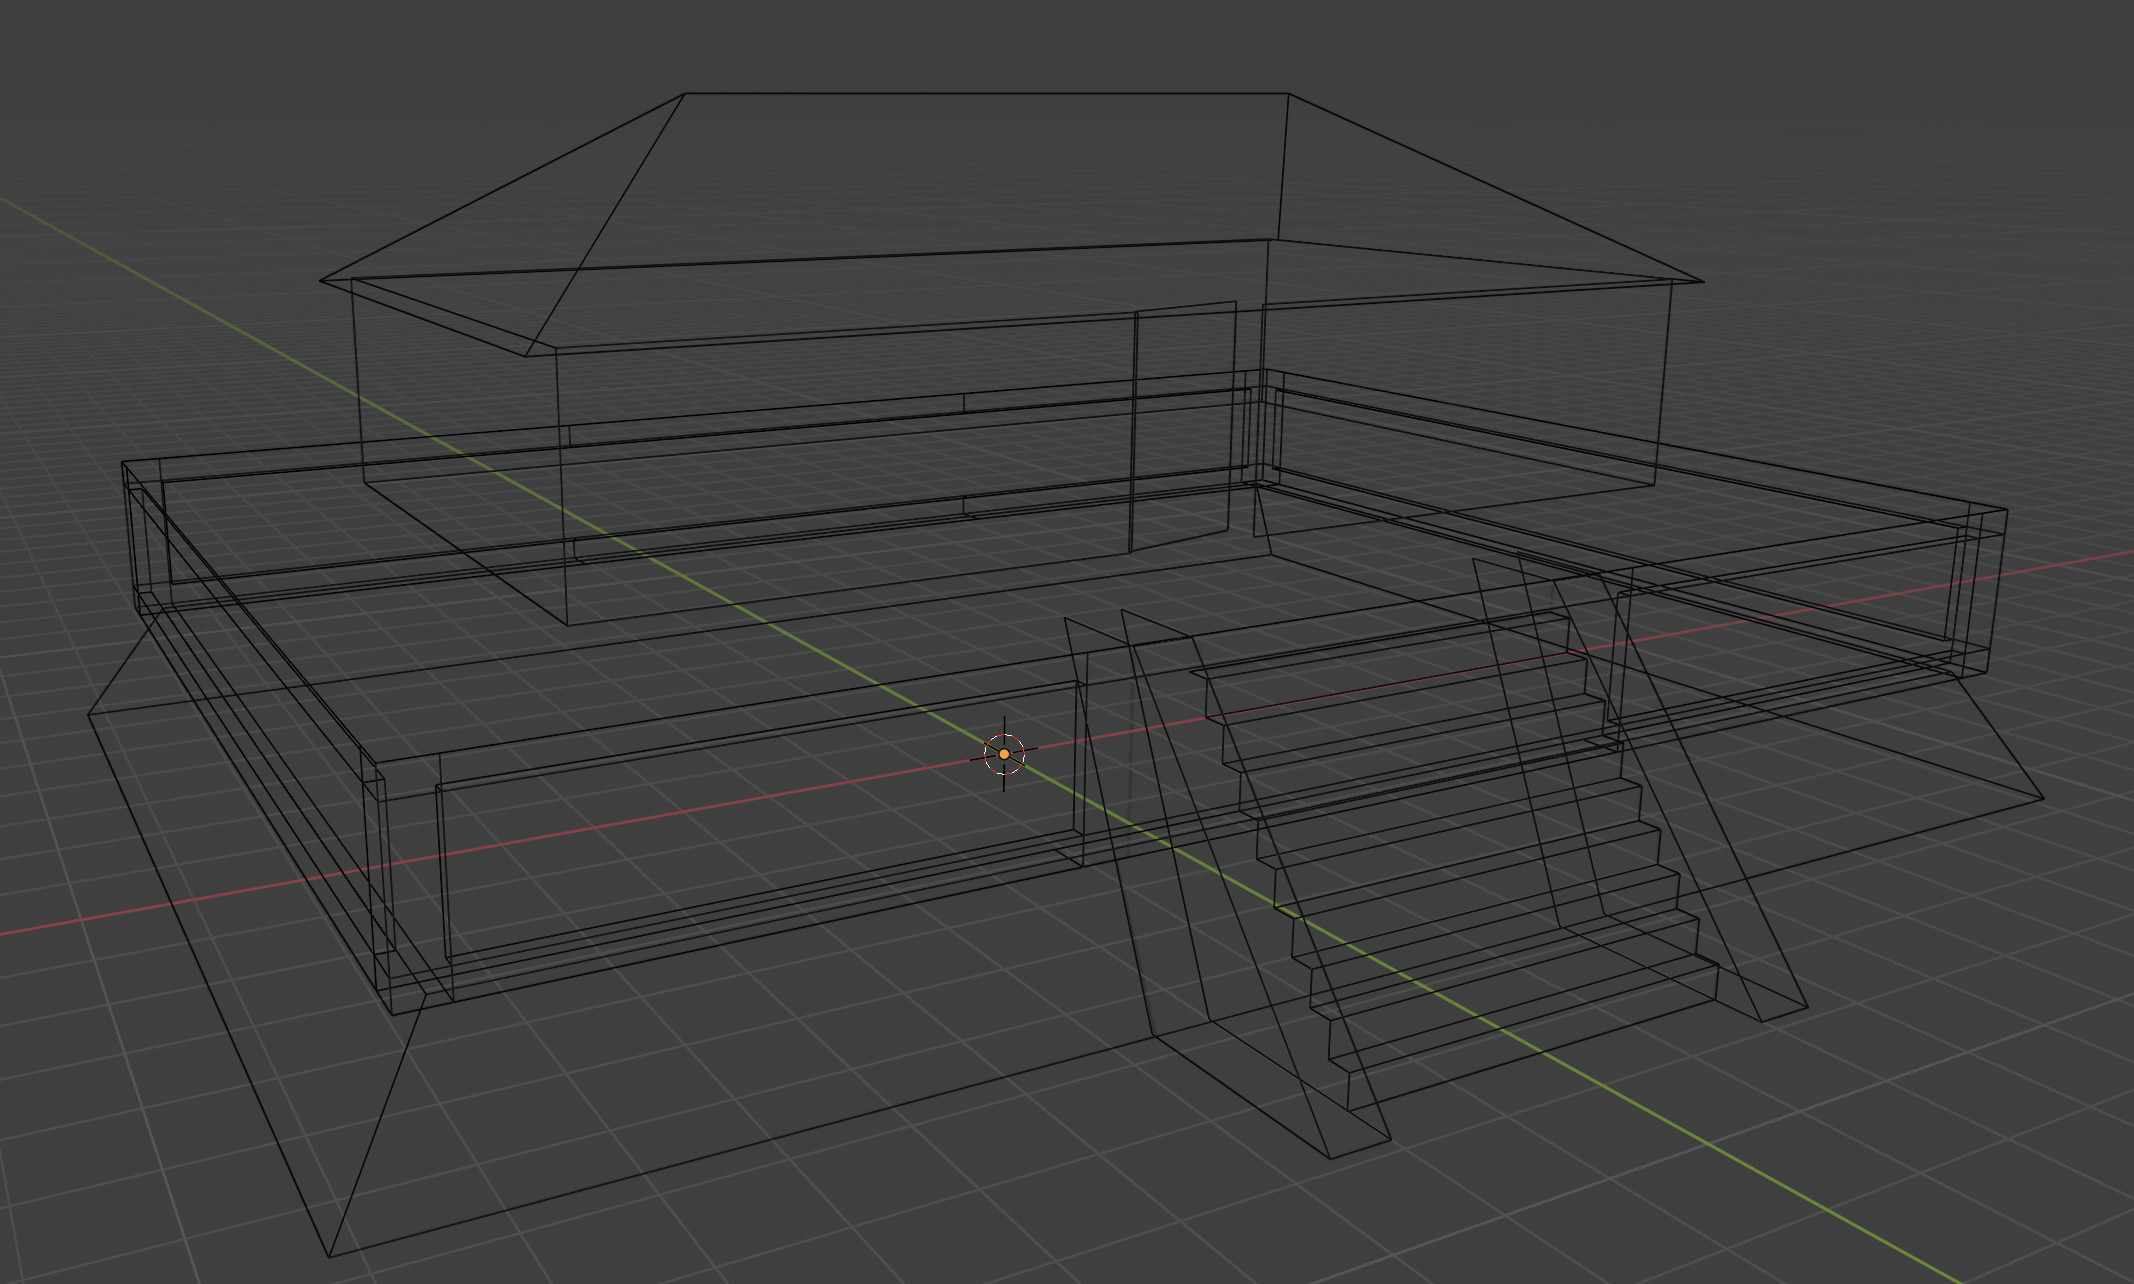
\includegraphics[width=0.85\linewidth]{resultados/figures/m7/m7_wireframe.png}
    \end{subfigure}\hfill
    \begin{subfigure}{0.48\textwidth}
        \centering
        \caption{Vista sólida sin texturas}
        \label{fig:m7-solid}
        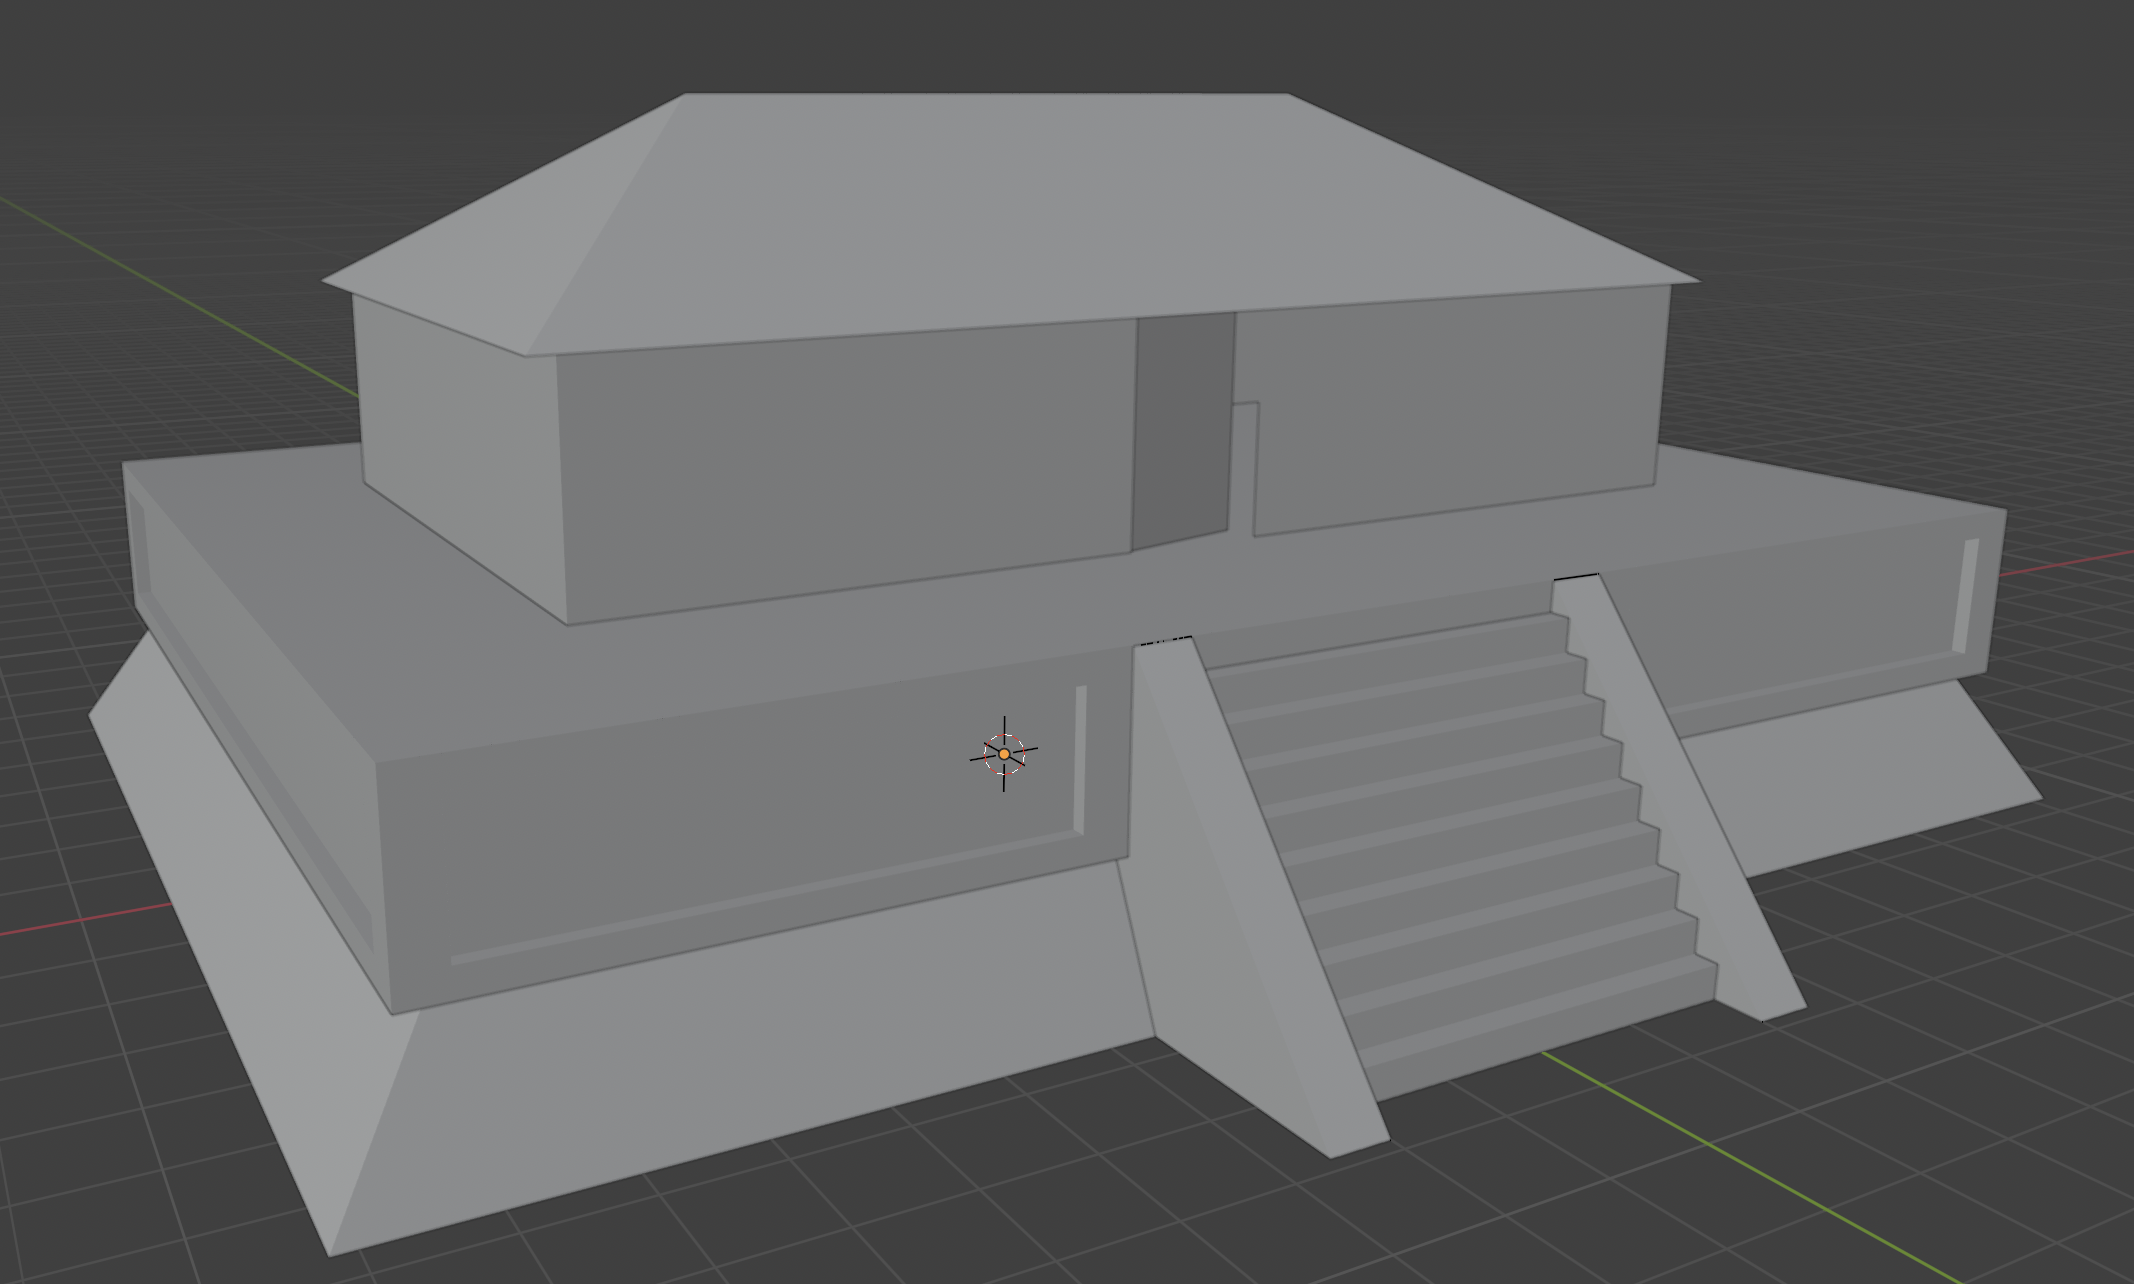
\includegraphics[width=0.85\linewidth]{resultados/figures/m7/m7_solid.png}
    \end{subfigure}

    \vspace{0.1em}

    % ----- Fila 2 -----
    \begin{subfigure}{0.48\textwidth}
        \centering
        \caption{Vista con materiales/texturas}
        \label{fig:m7-textured}
        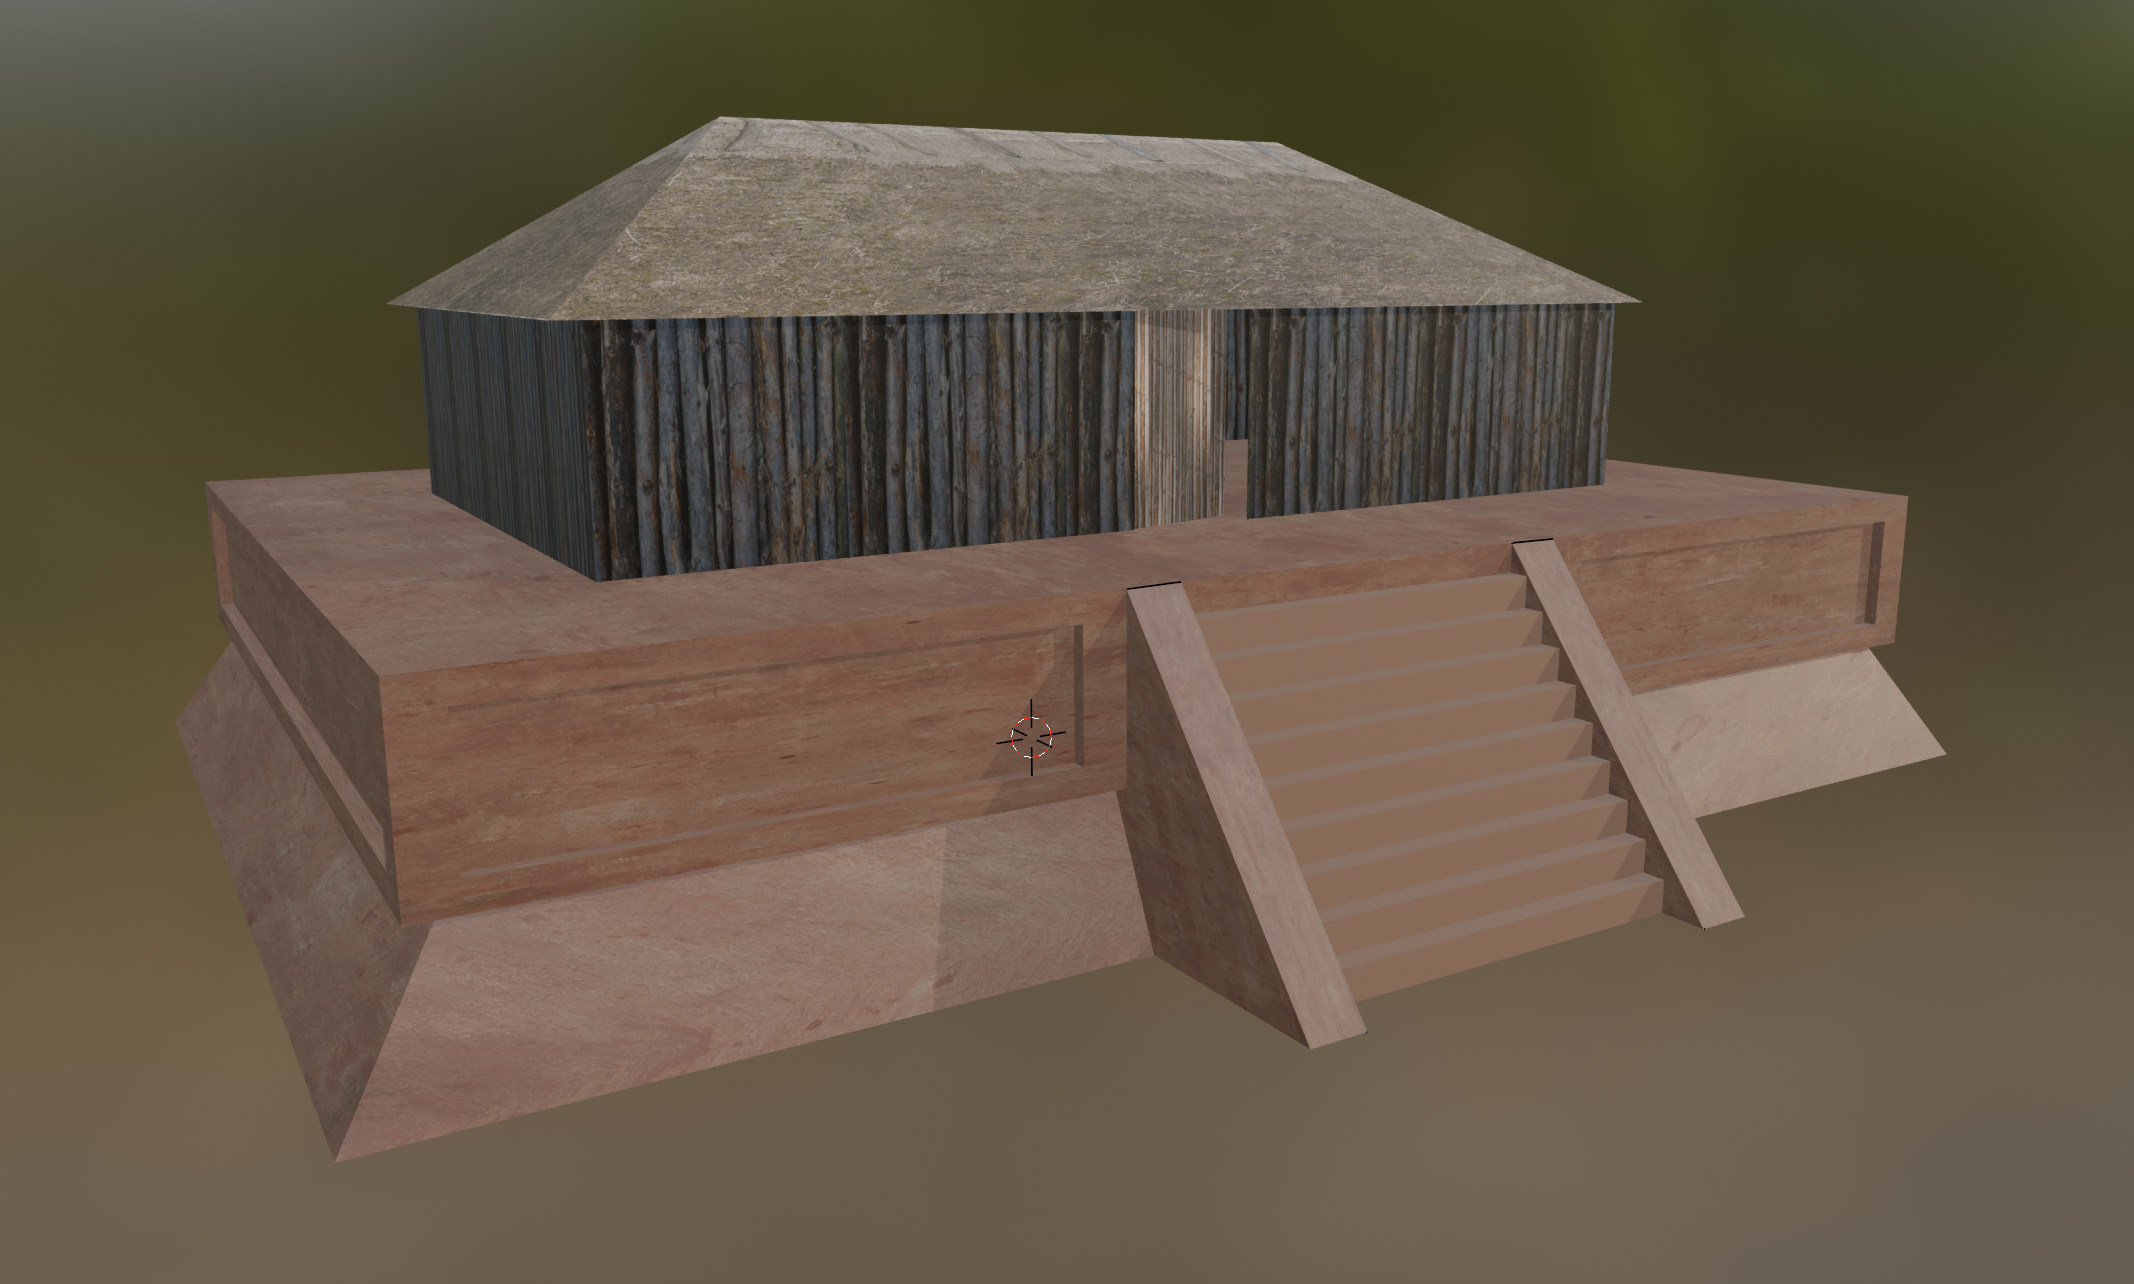
\includegraphics[width=0.85\linewidth]{resultados/figures/m7/m7_textured_viewport.png}
    \end{subfigure}
\end{figure}


\begin{figure}[!htbp]
    \centering
    \caption{Montículo 7 visualizado en la aplicación de realidad aumentada, mostrando la reconstrucción superpuesta en el entorno real del parque arqueológico}
    \label{fig:m7-ar}
    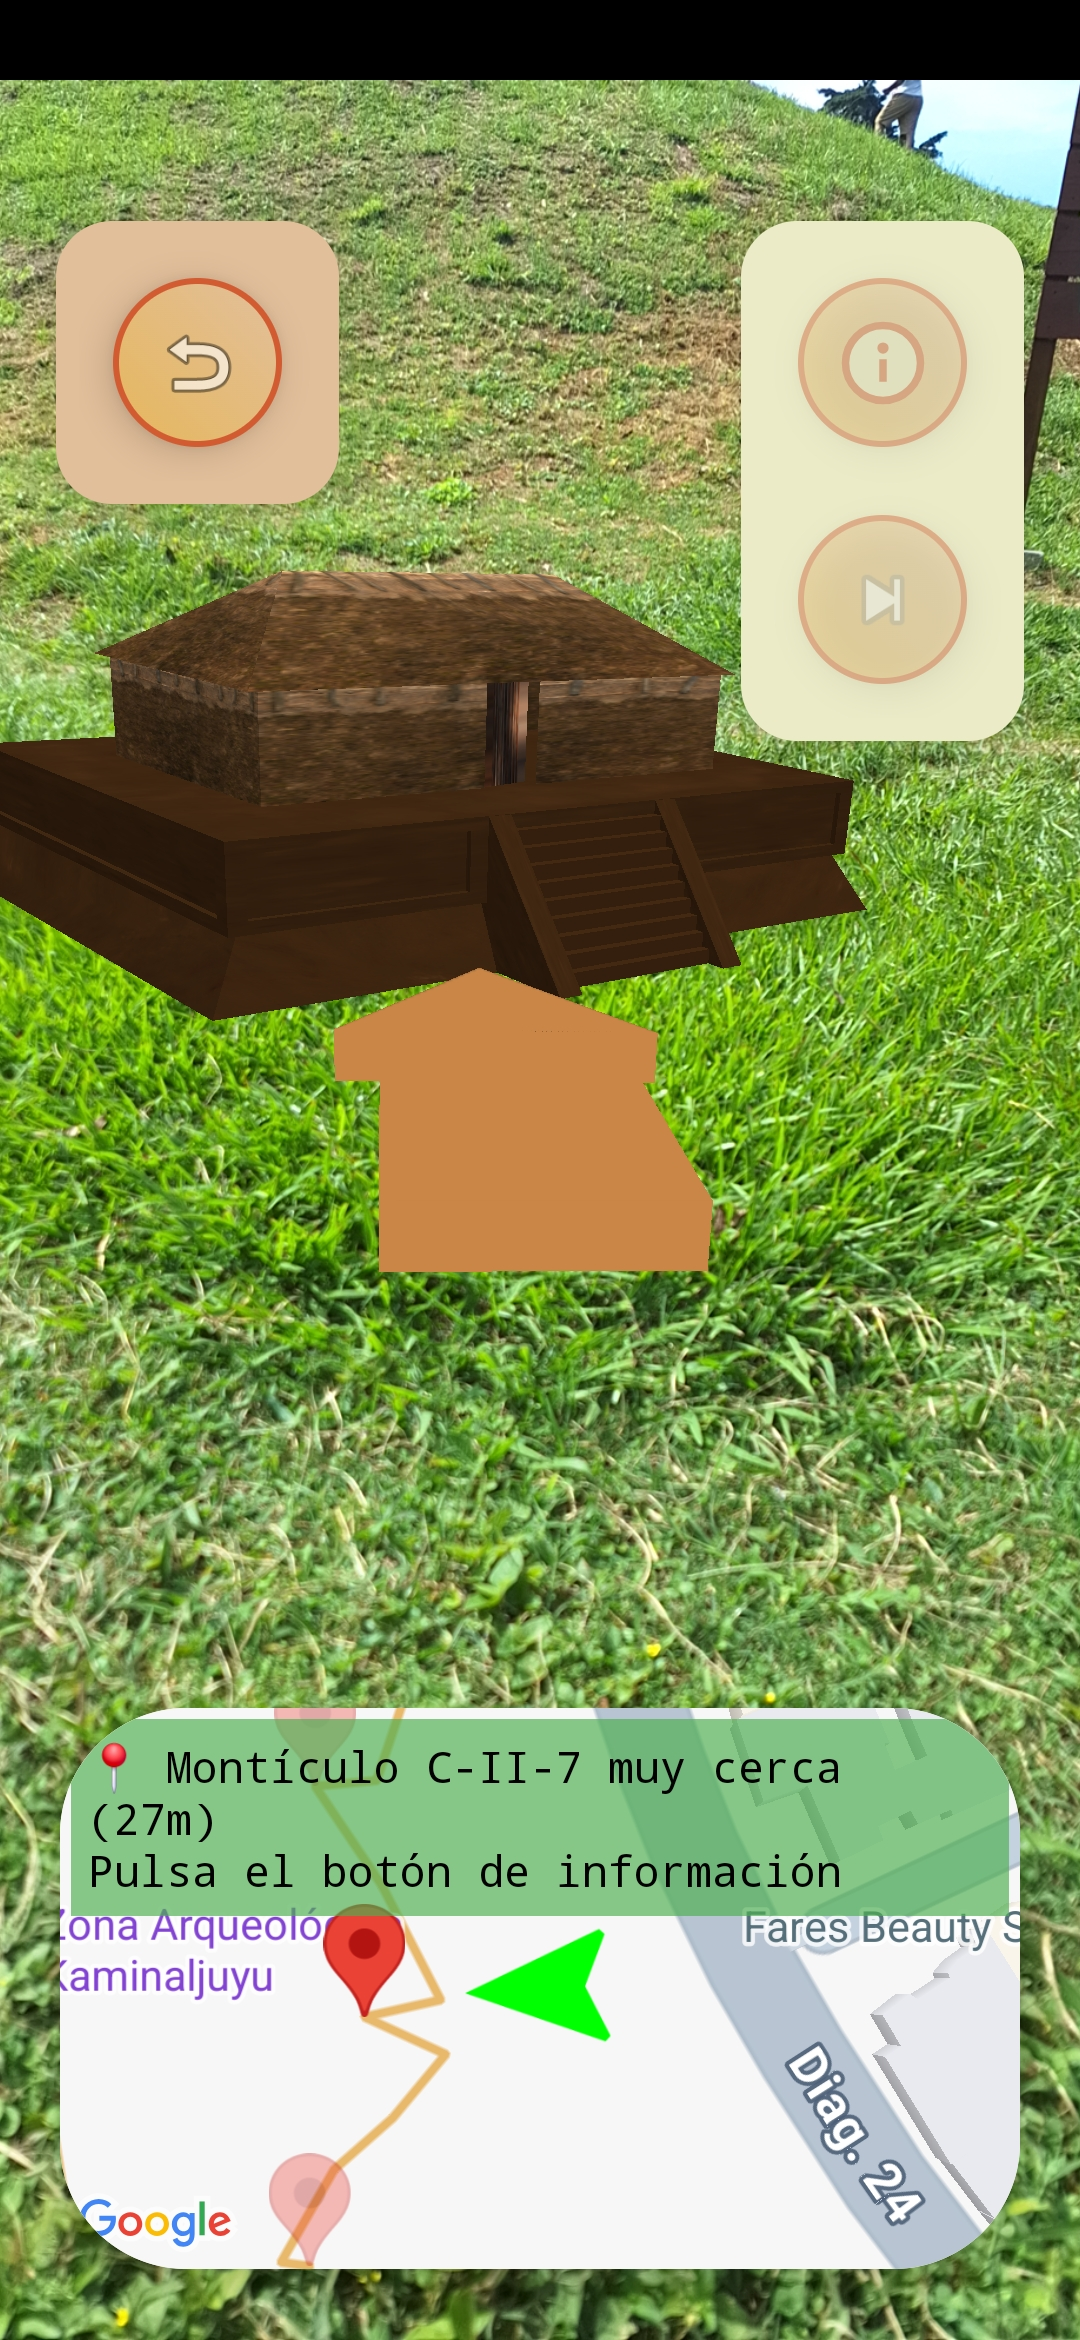
\includegraphics[width=0.28\linewidth]{resultados/figures/m7/m7_ar.jpg}
\end{figure}
\FloatBarrier
\clearpage
\FloatBarrier
\subsection{Montículo 12}

\begin{figure}[!htbp]
    \centering
    \caption{Montículo 12, panel de vistas}
    \label{fig:m12-panel}
    % ----- Fila 1 -----
    \begin{subfigure}{0.48\textwidth}
        \centering
        \caption{Vista en malla (wireframe)}
        \label{fig:m12-wire}
        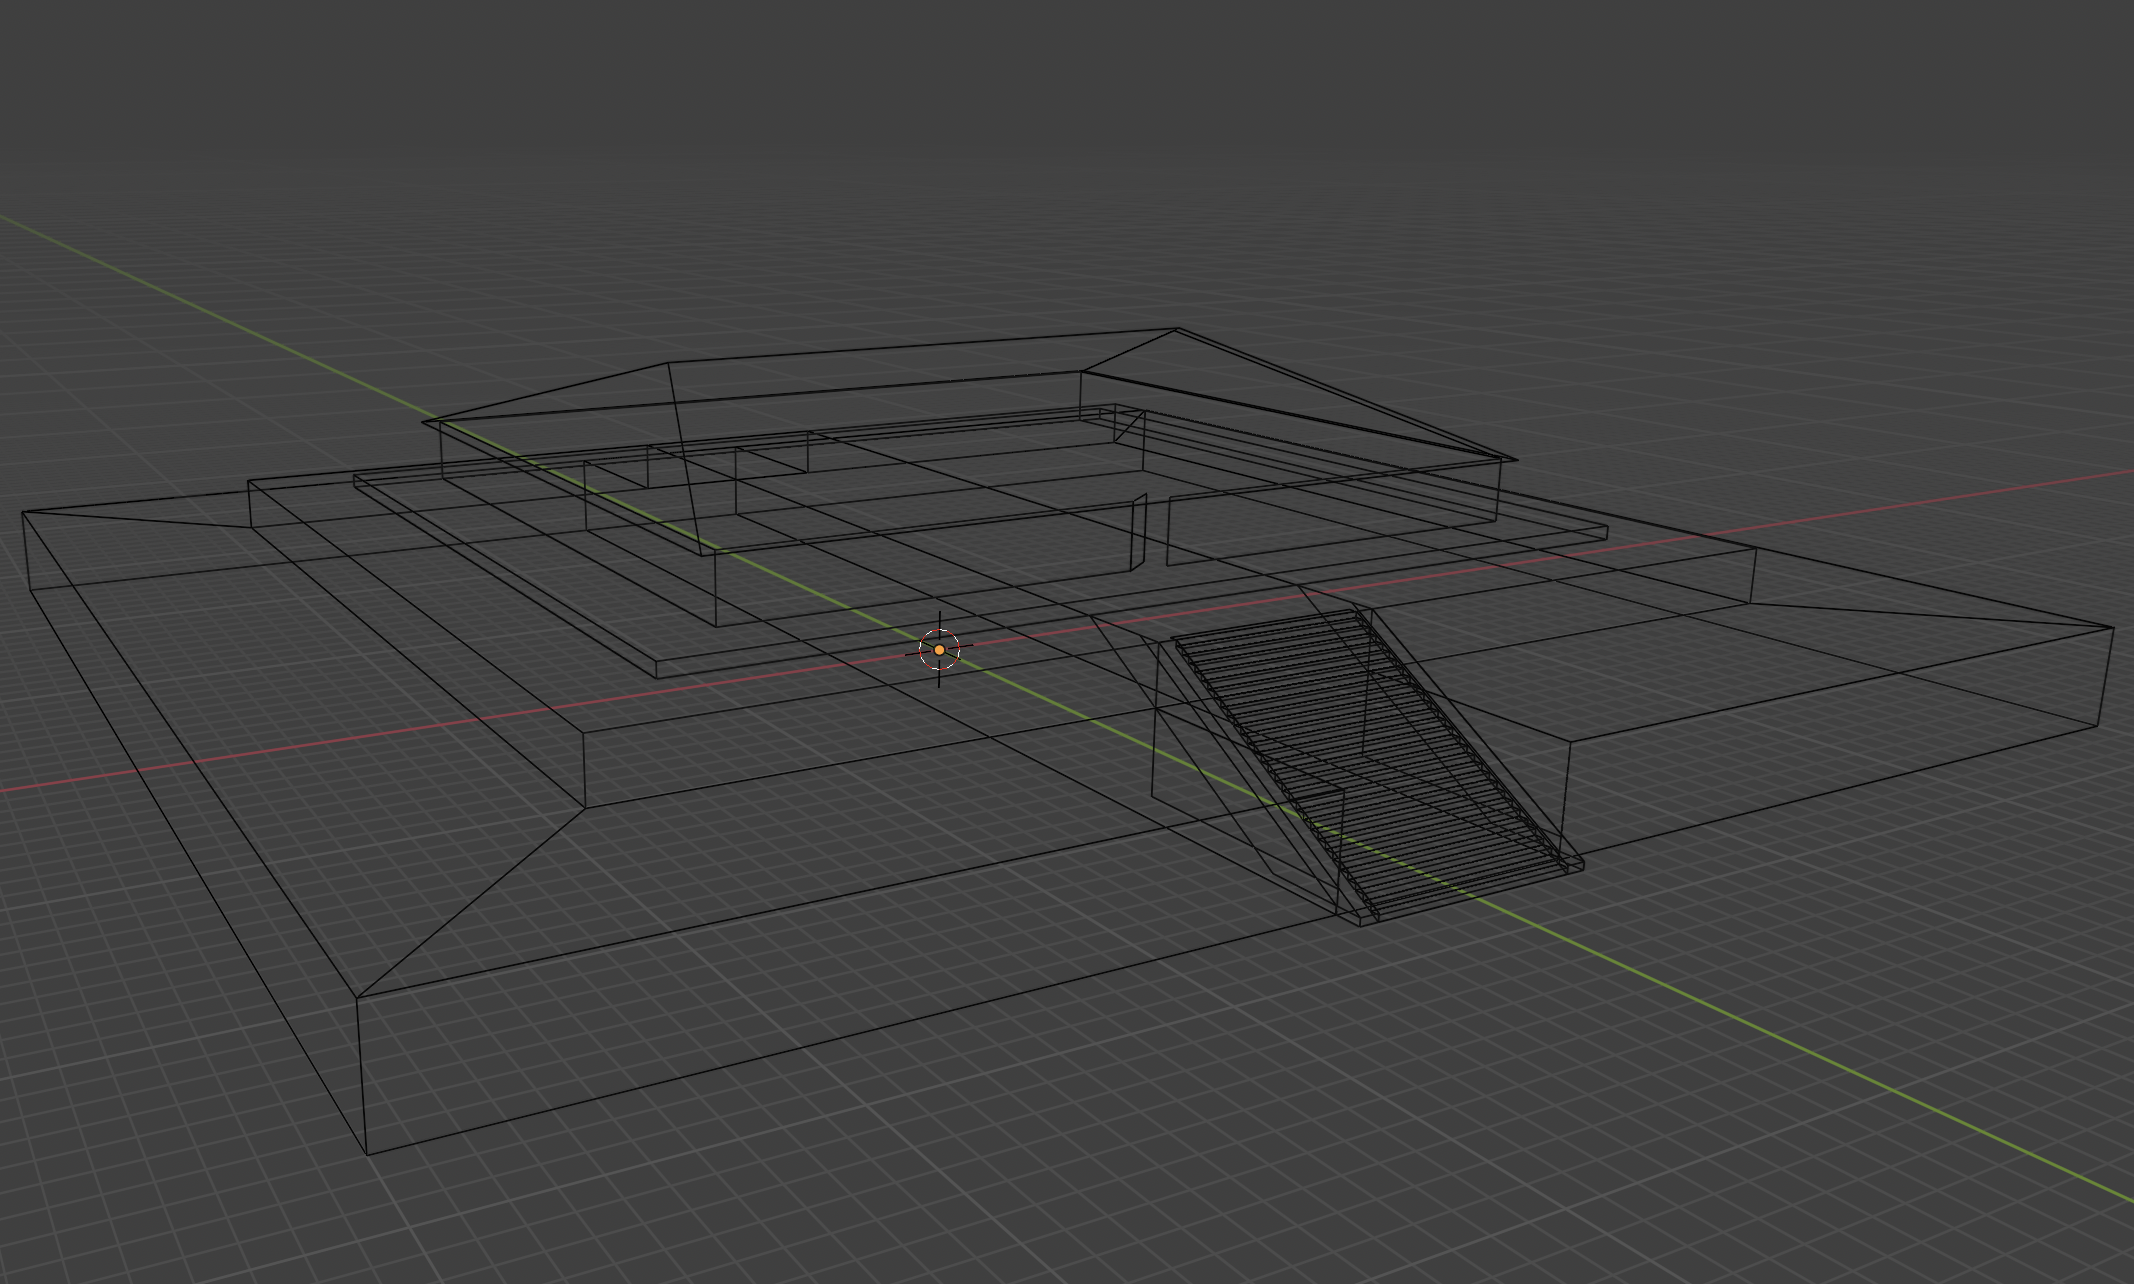
\includegraphics[width=0.85\linewidth]{resultados/figures/m12/m12_wireframe.png}
    \end{subfigure}\hfill
    \begin{subfigure}{0.48\textwidth}
        \centering
        \caption{Vista sólida sin texturas}
        \label{fig:m12-solid}
        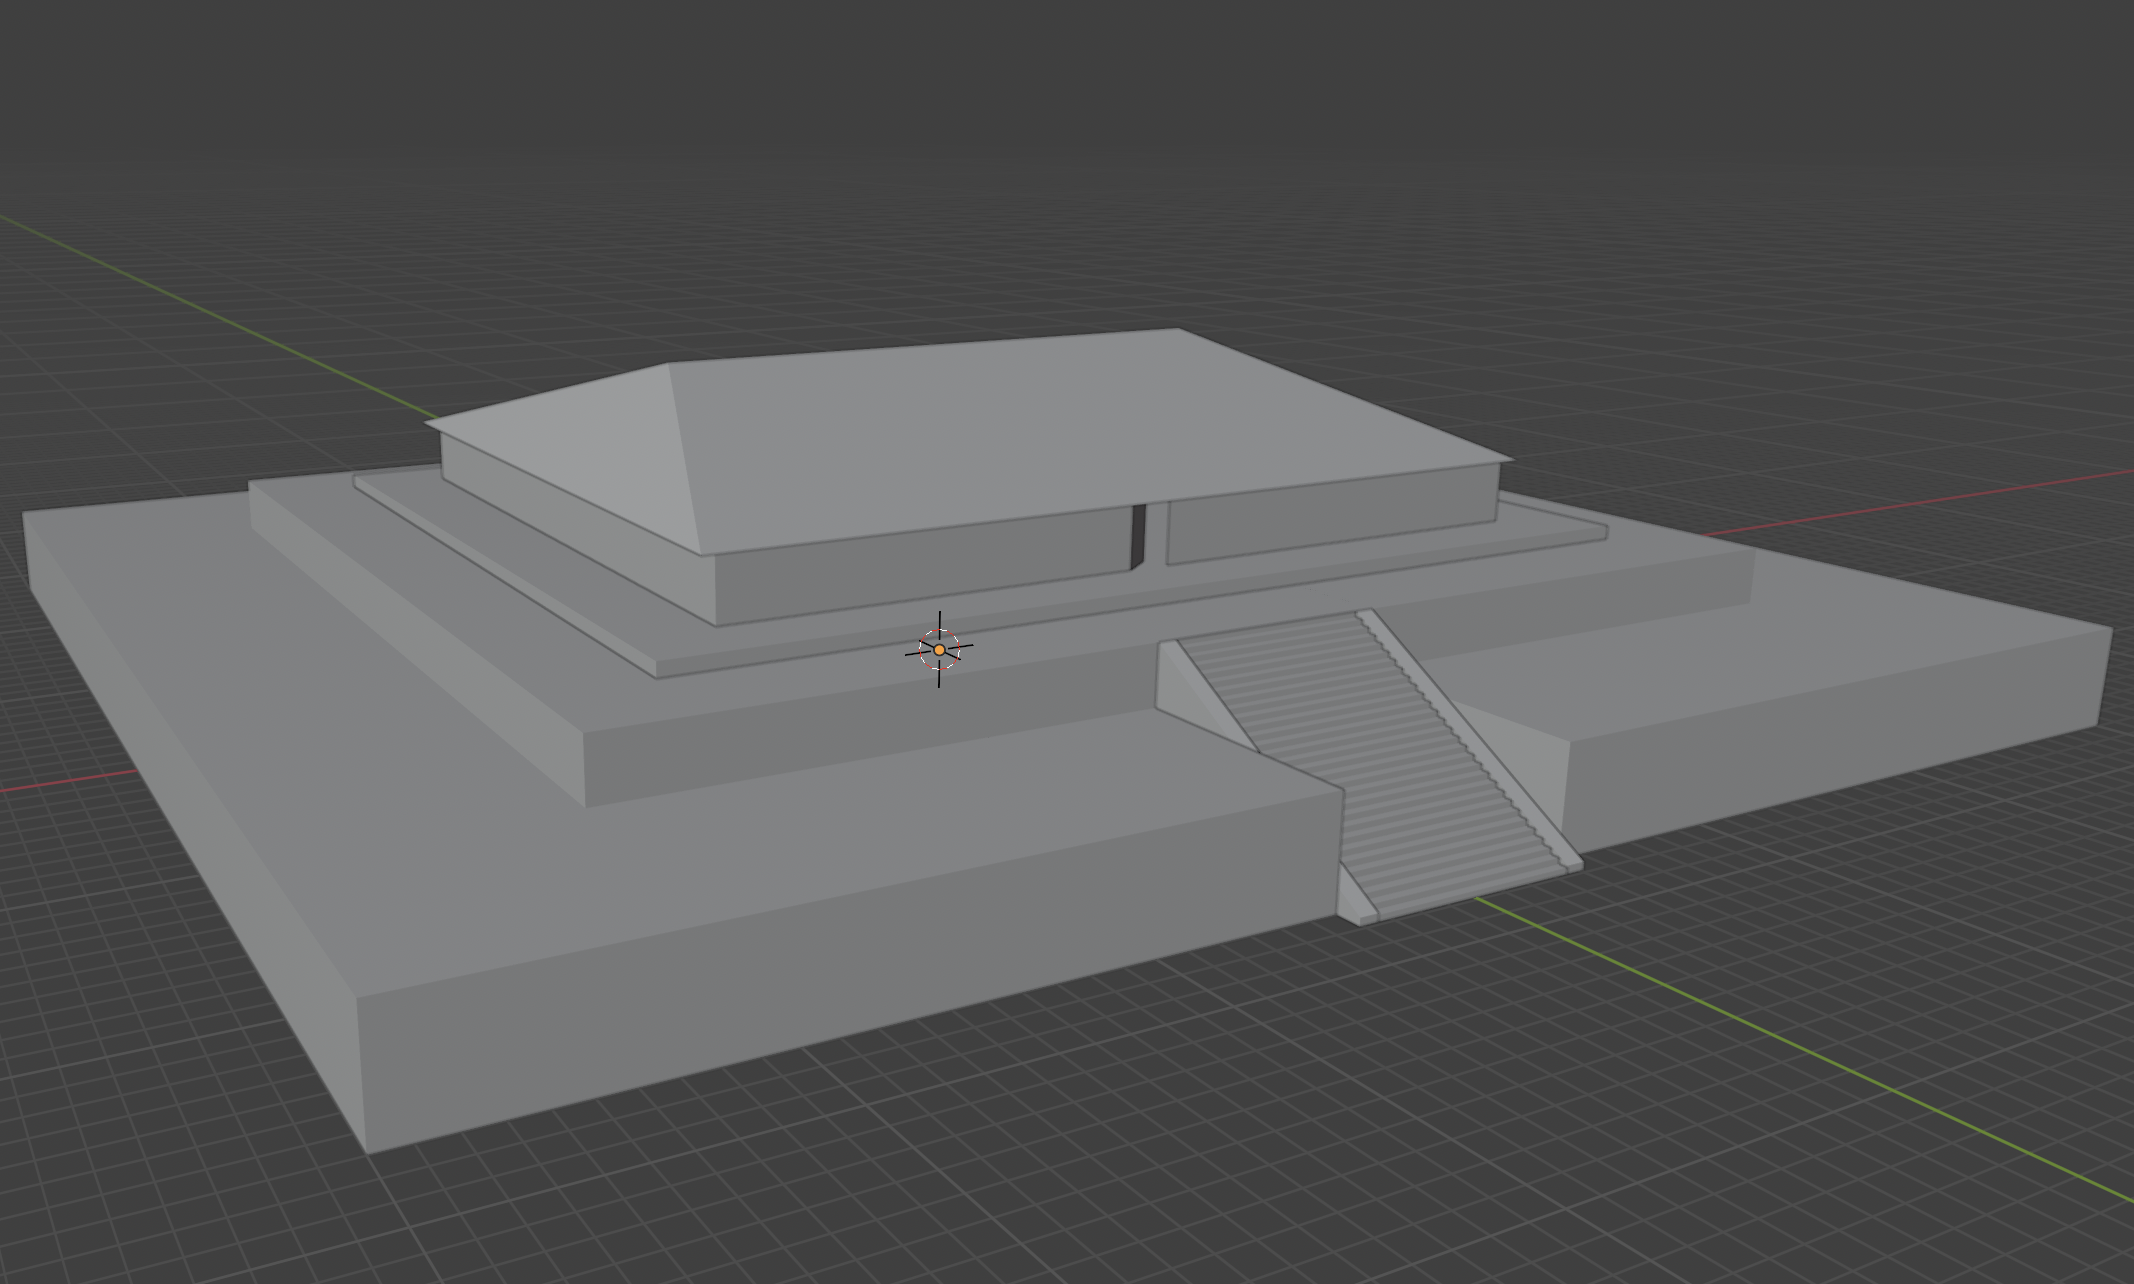
\includegraphics[width=0.85\linewidth]{resultados/figures/m12/m12_solid.png}
    \end{subfigure}

    \vspace{0.1em}

    % ----- Fila 2 -----
    \begin{subfigure}{0.48\textwidth}
        \centering
        \caption{Vista con materiales/texturas}
        \label{fig:m12-textured}
        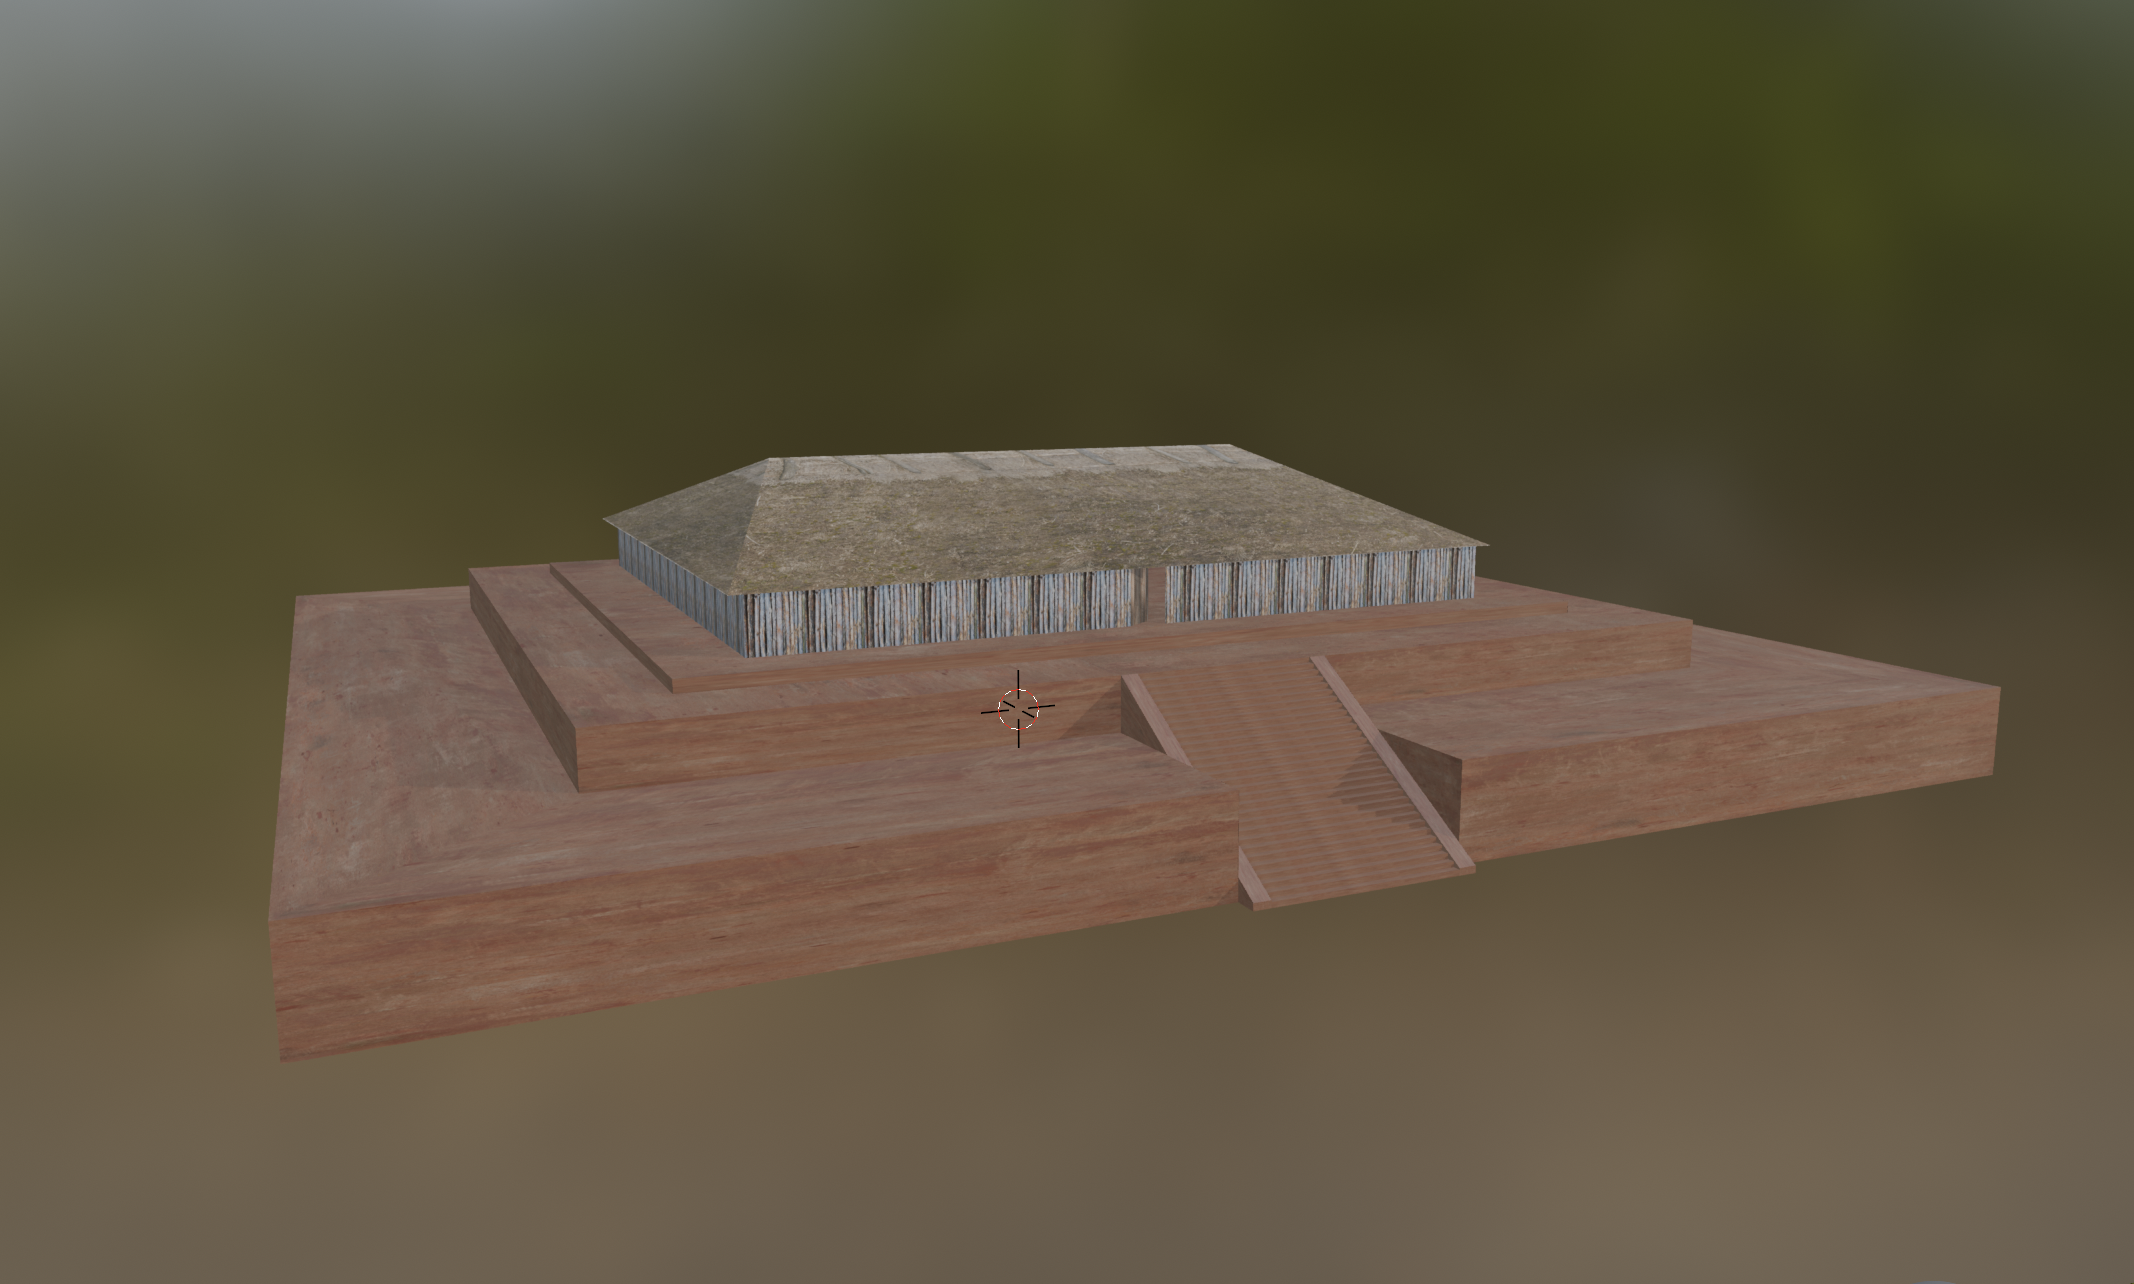
\includegraphics[width=0.85\linewidth]{resultados/figures/m12/m12_textured_viewport.png}
    \end{subfigure}
\end{figure}

\begin{figure}[!htbp]
    \centering
    \caption{Montículo 12 visualizado en la aplicación de realidad aumentada, mostrando la reconstrucción superpuesta en el entorno real del parque arqueológico}
    \label{fig:m12-ar}
    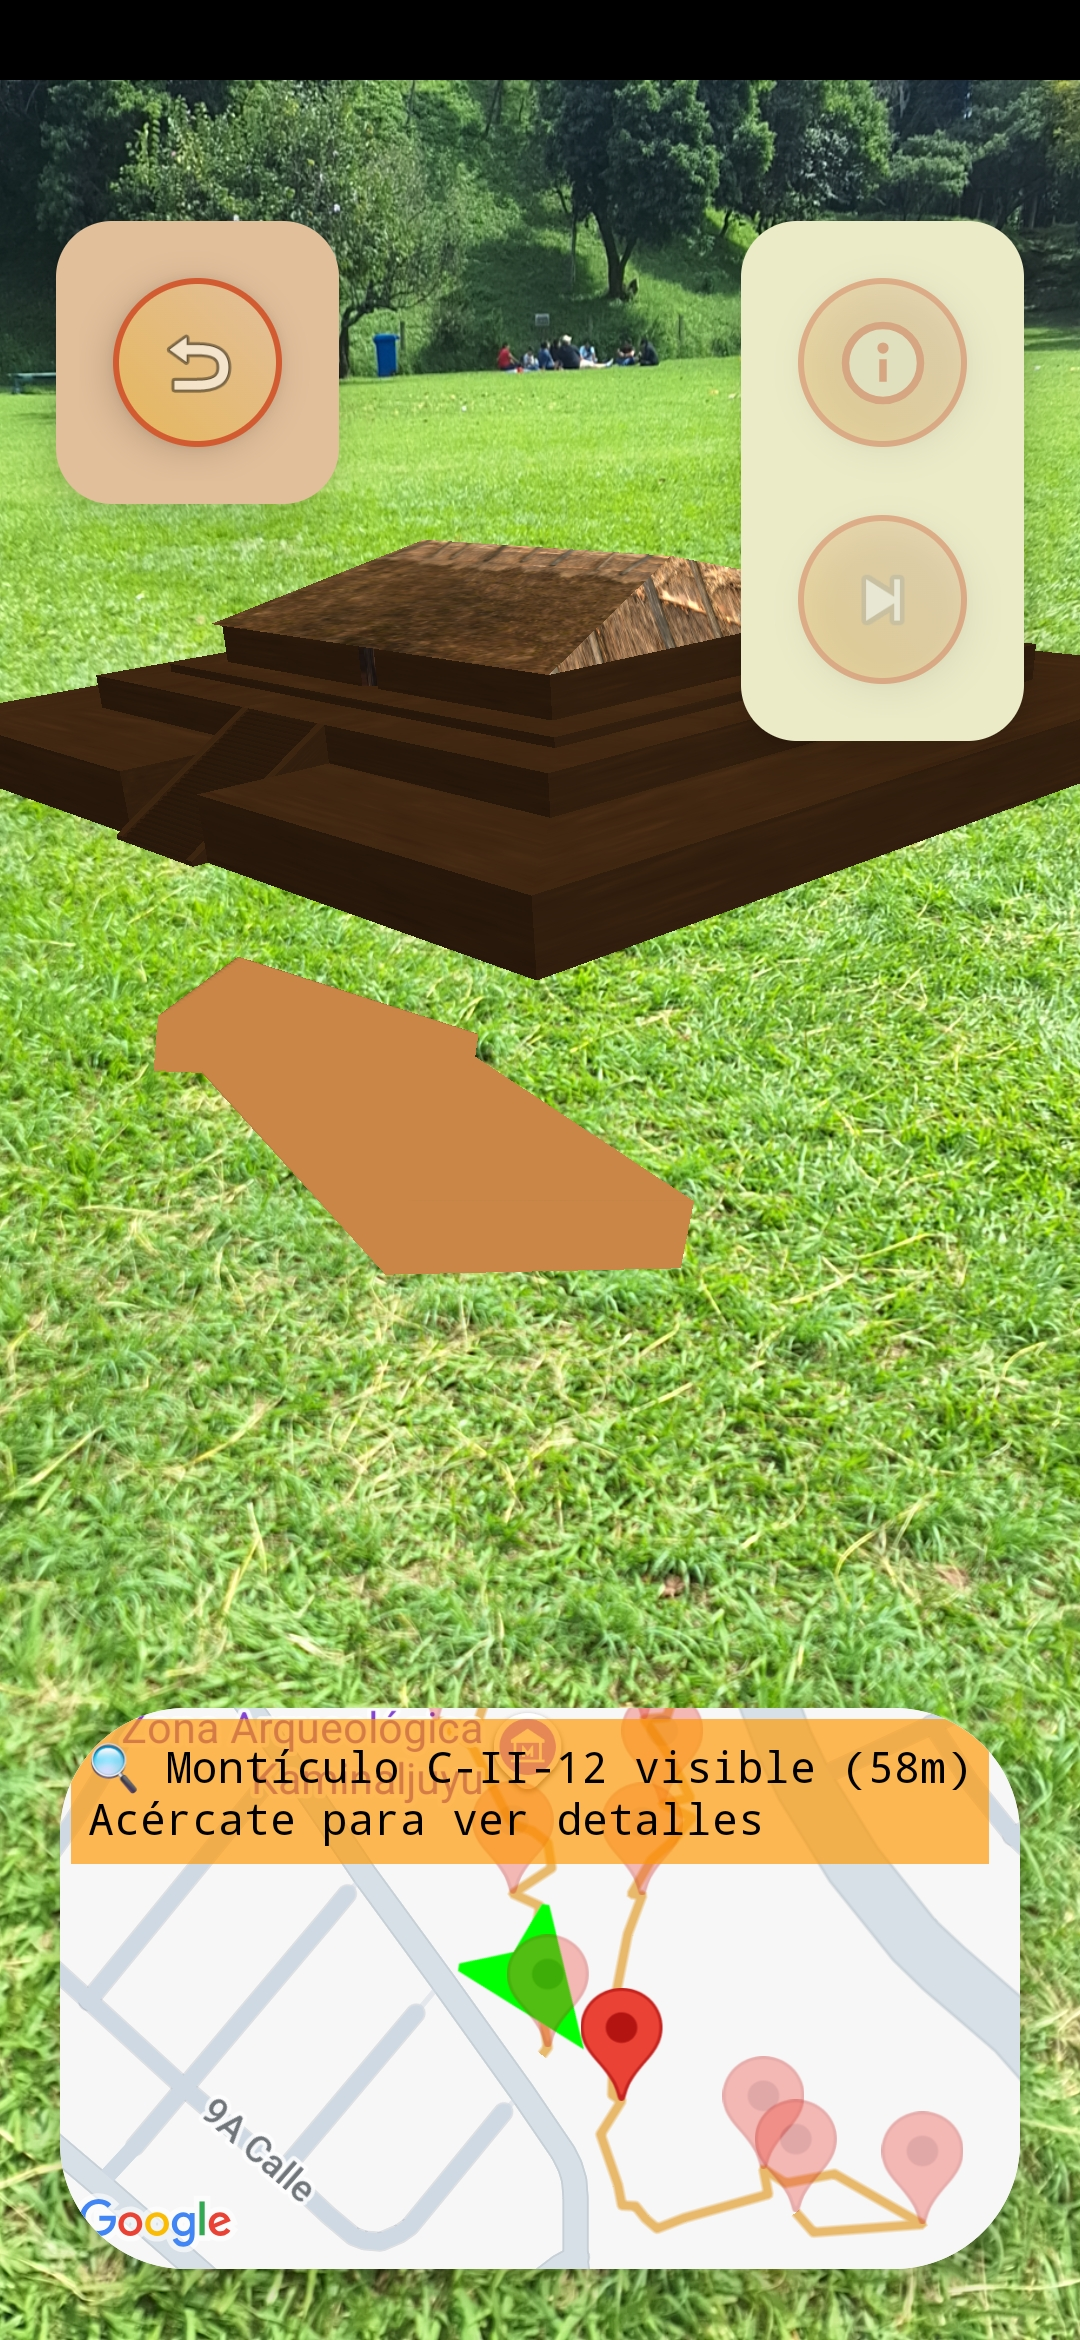
\includegraphics[width=0.28\linewidth]{resultados/figures/m12/m12_ar.jpg}
\end{figure}
\FloatBarrier
\clearpage
\FloatBarrier
\subsection{Montículo 13}

\begin{figure}[!htbp]
    \centering
    \caption{Montículo 13, panel de vistas}
    \label{fig:m13-panel}
    % ----- Fila 1 -----
    \begin{subfigure}{0.48\textwidth}
        \centering
        \caption{Vista en malla (wireframe)}
        \label{fig:m13-wire}
        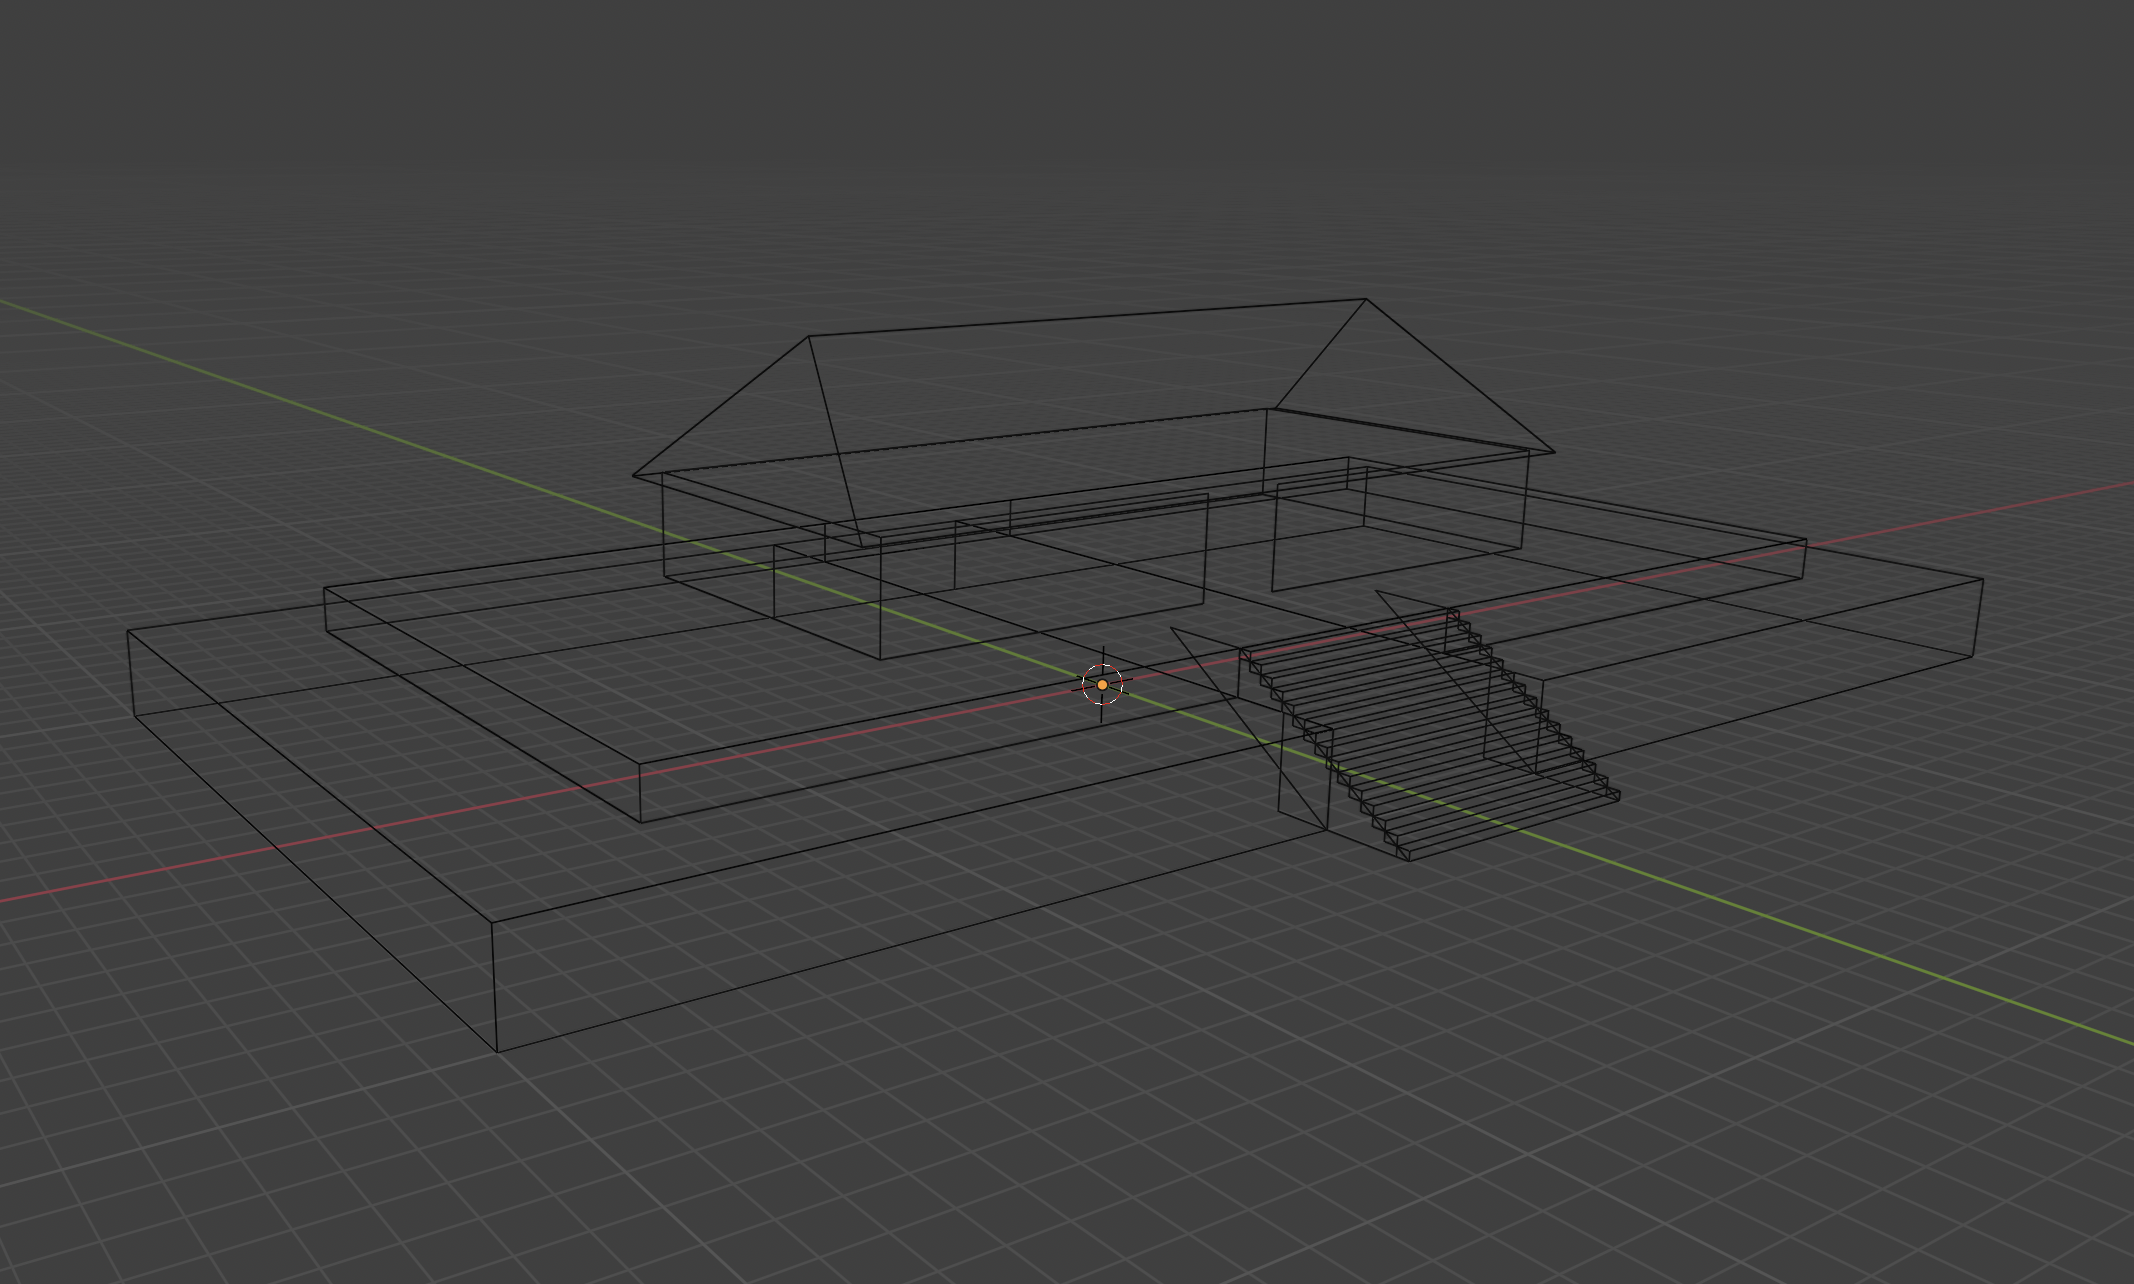
\includegraphics[width=0.85\linewidth]{resultados/figures/m13/m13_wireframe.png}
    \end{subfigure}\hfill
    \begin{subfigure}{0.48\textwidth}
        \centering
        \caption{Vista sólida sin texturas}
        \label{fig:m13-solid}
        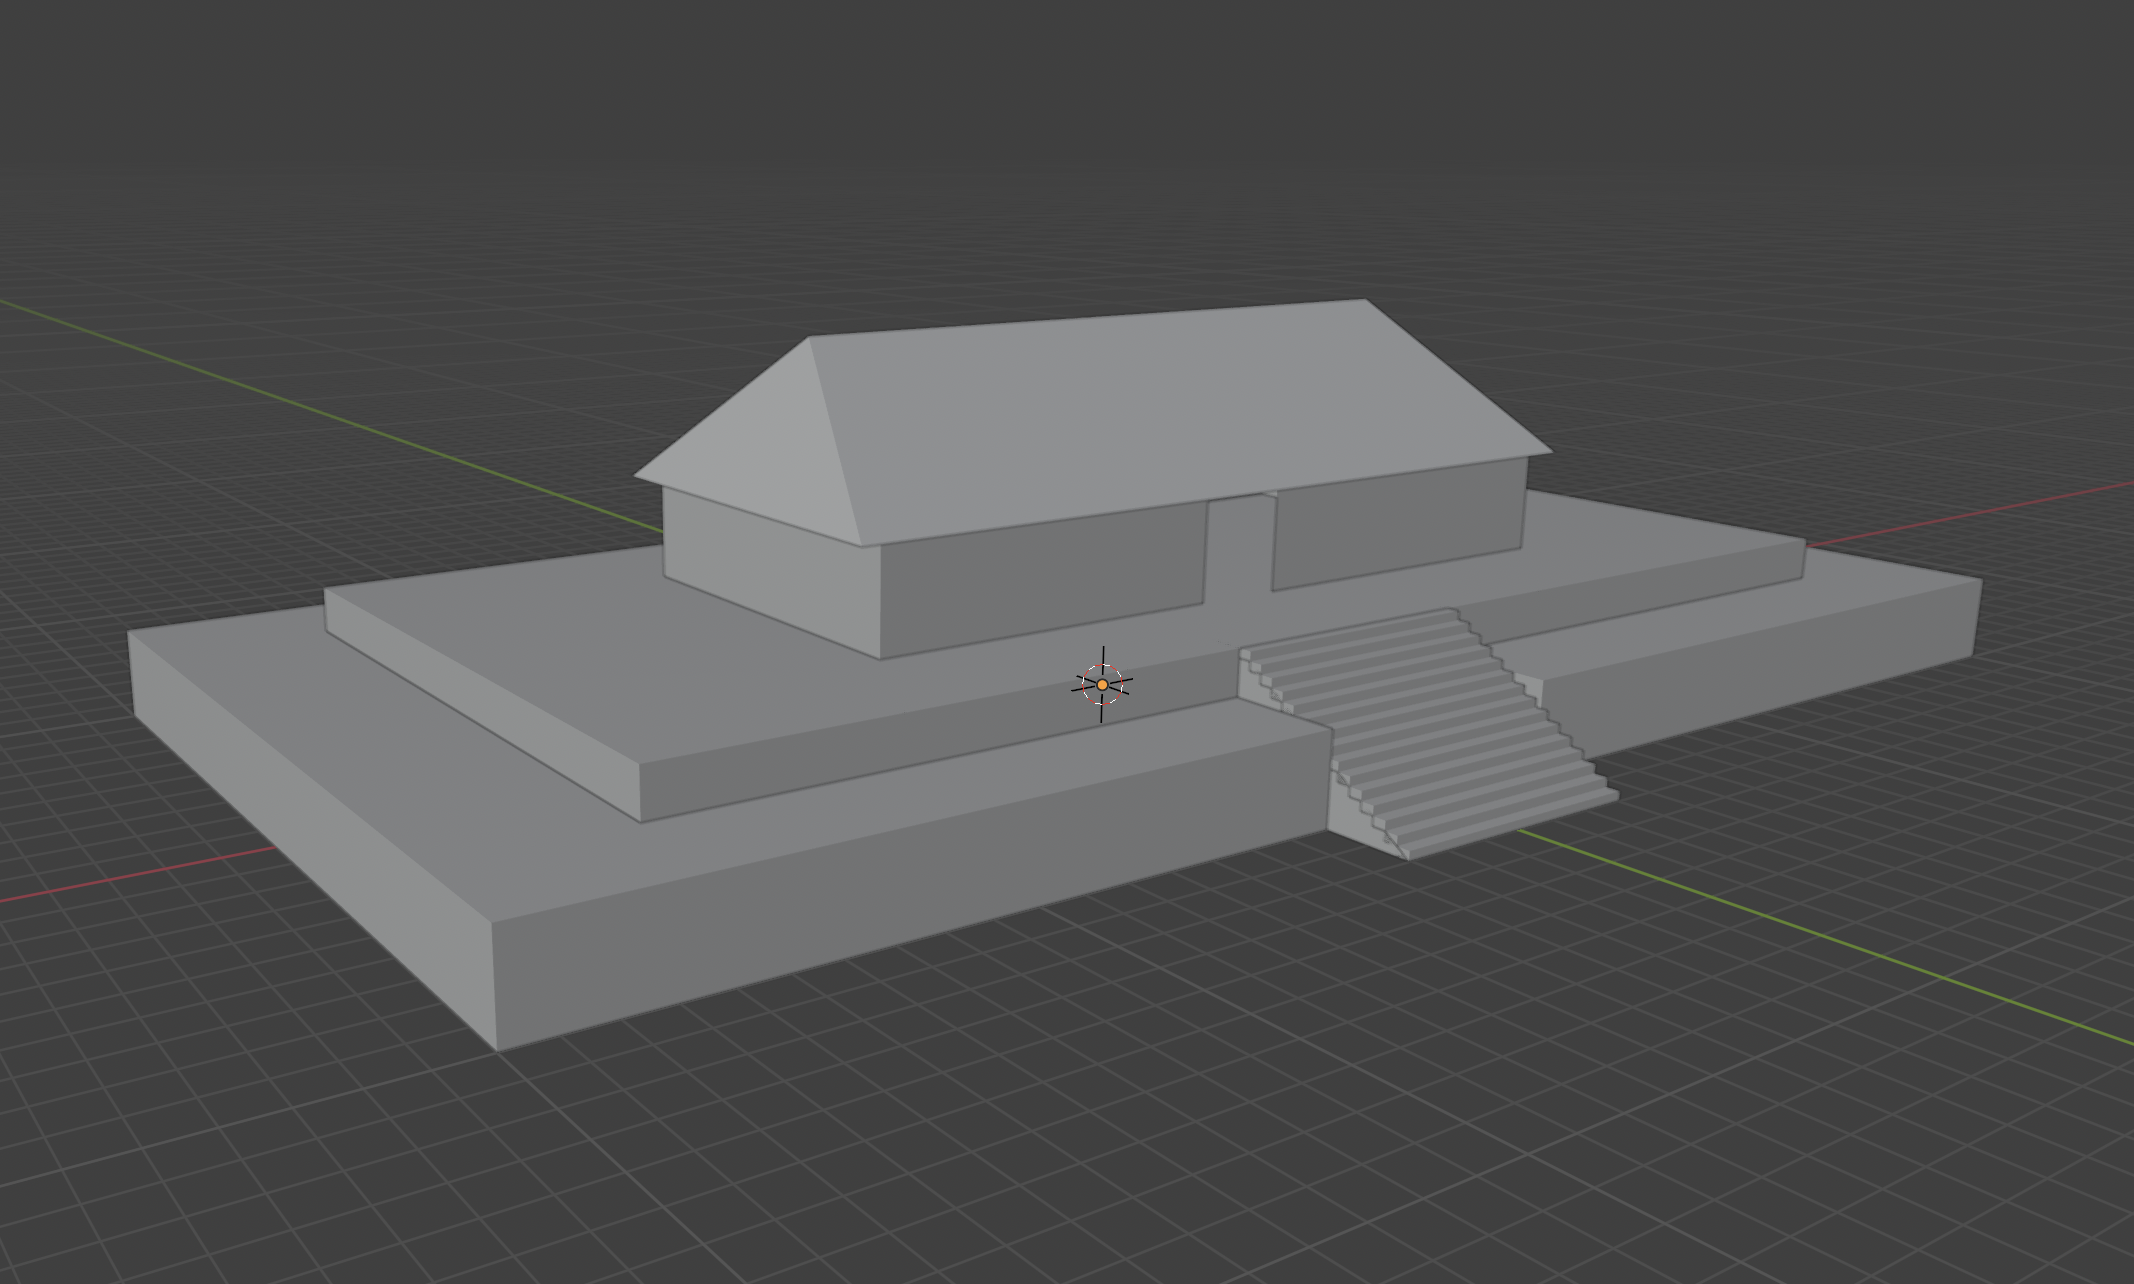
\includegraphics[width=0.85\linewidth]{resultados/figures/m13/m13_solid.png}
    \end{subfigure}

    \vspace{0.5em}

    % ----- Fila 2 -----
    \begin{subfigure}{0.48\textwidth}
        \centering
        \caption{Vista con materiales/texturas}
        \label{fig:m13-textured}
        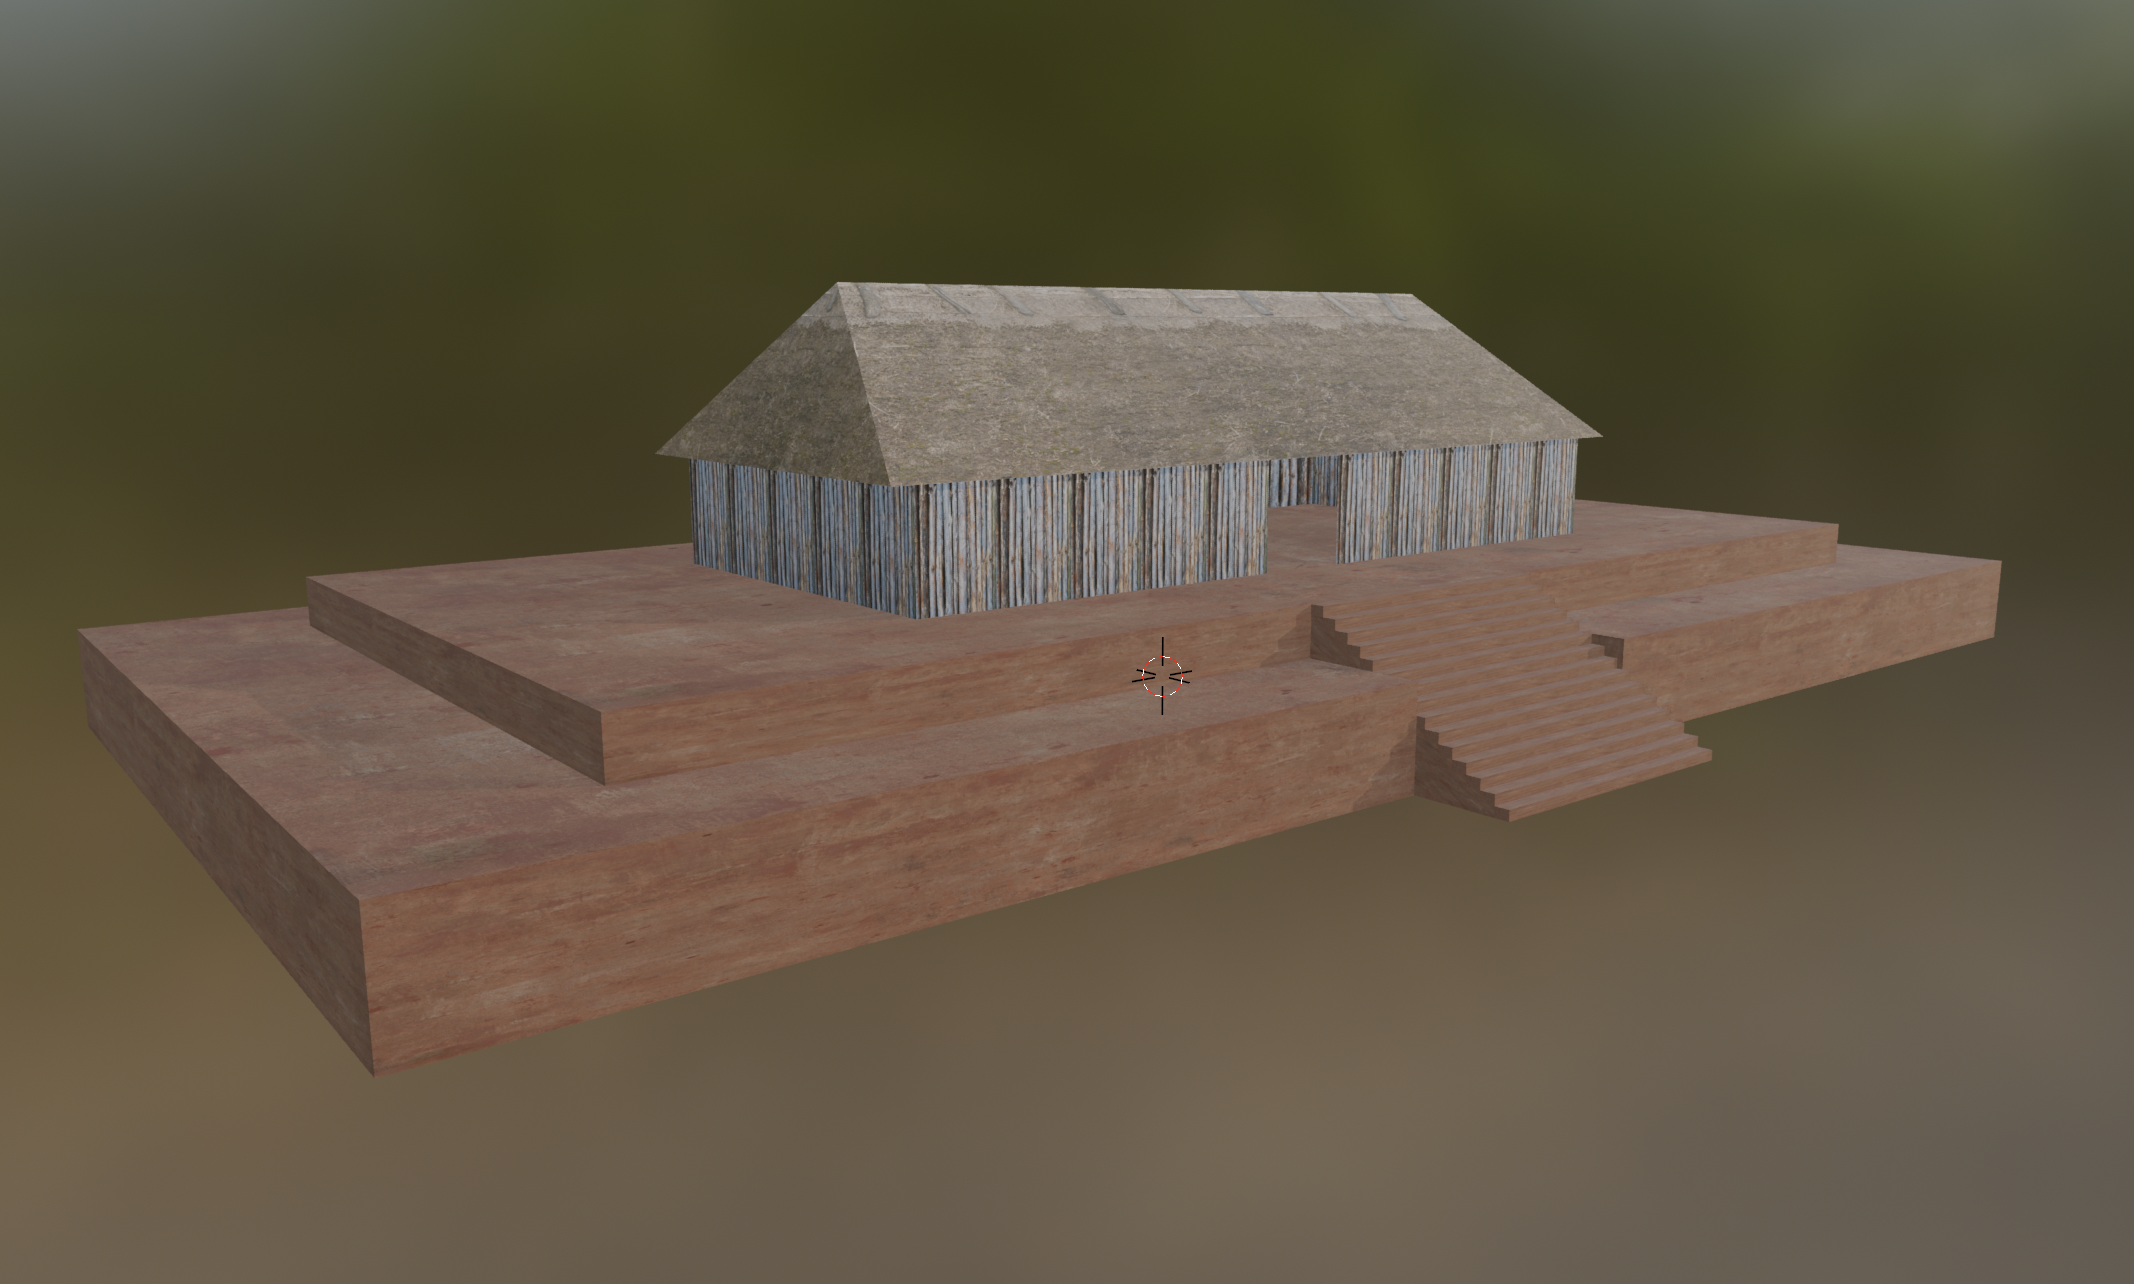
\includegraphics[width=0.85\linewidth]{resultados/figures/m13/m13_textured_viewport.png}
    \end{subfigure}
\end{figure}

\begin{figure}[!htbp]
    \centering
    \caption{Montículo 13 visualizado en la aplicación de realidad aumentada, mostrando la reconstrucción superpuesta en el entorno real del parque arqueológico}
    \label{fig:m13-ar}
    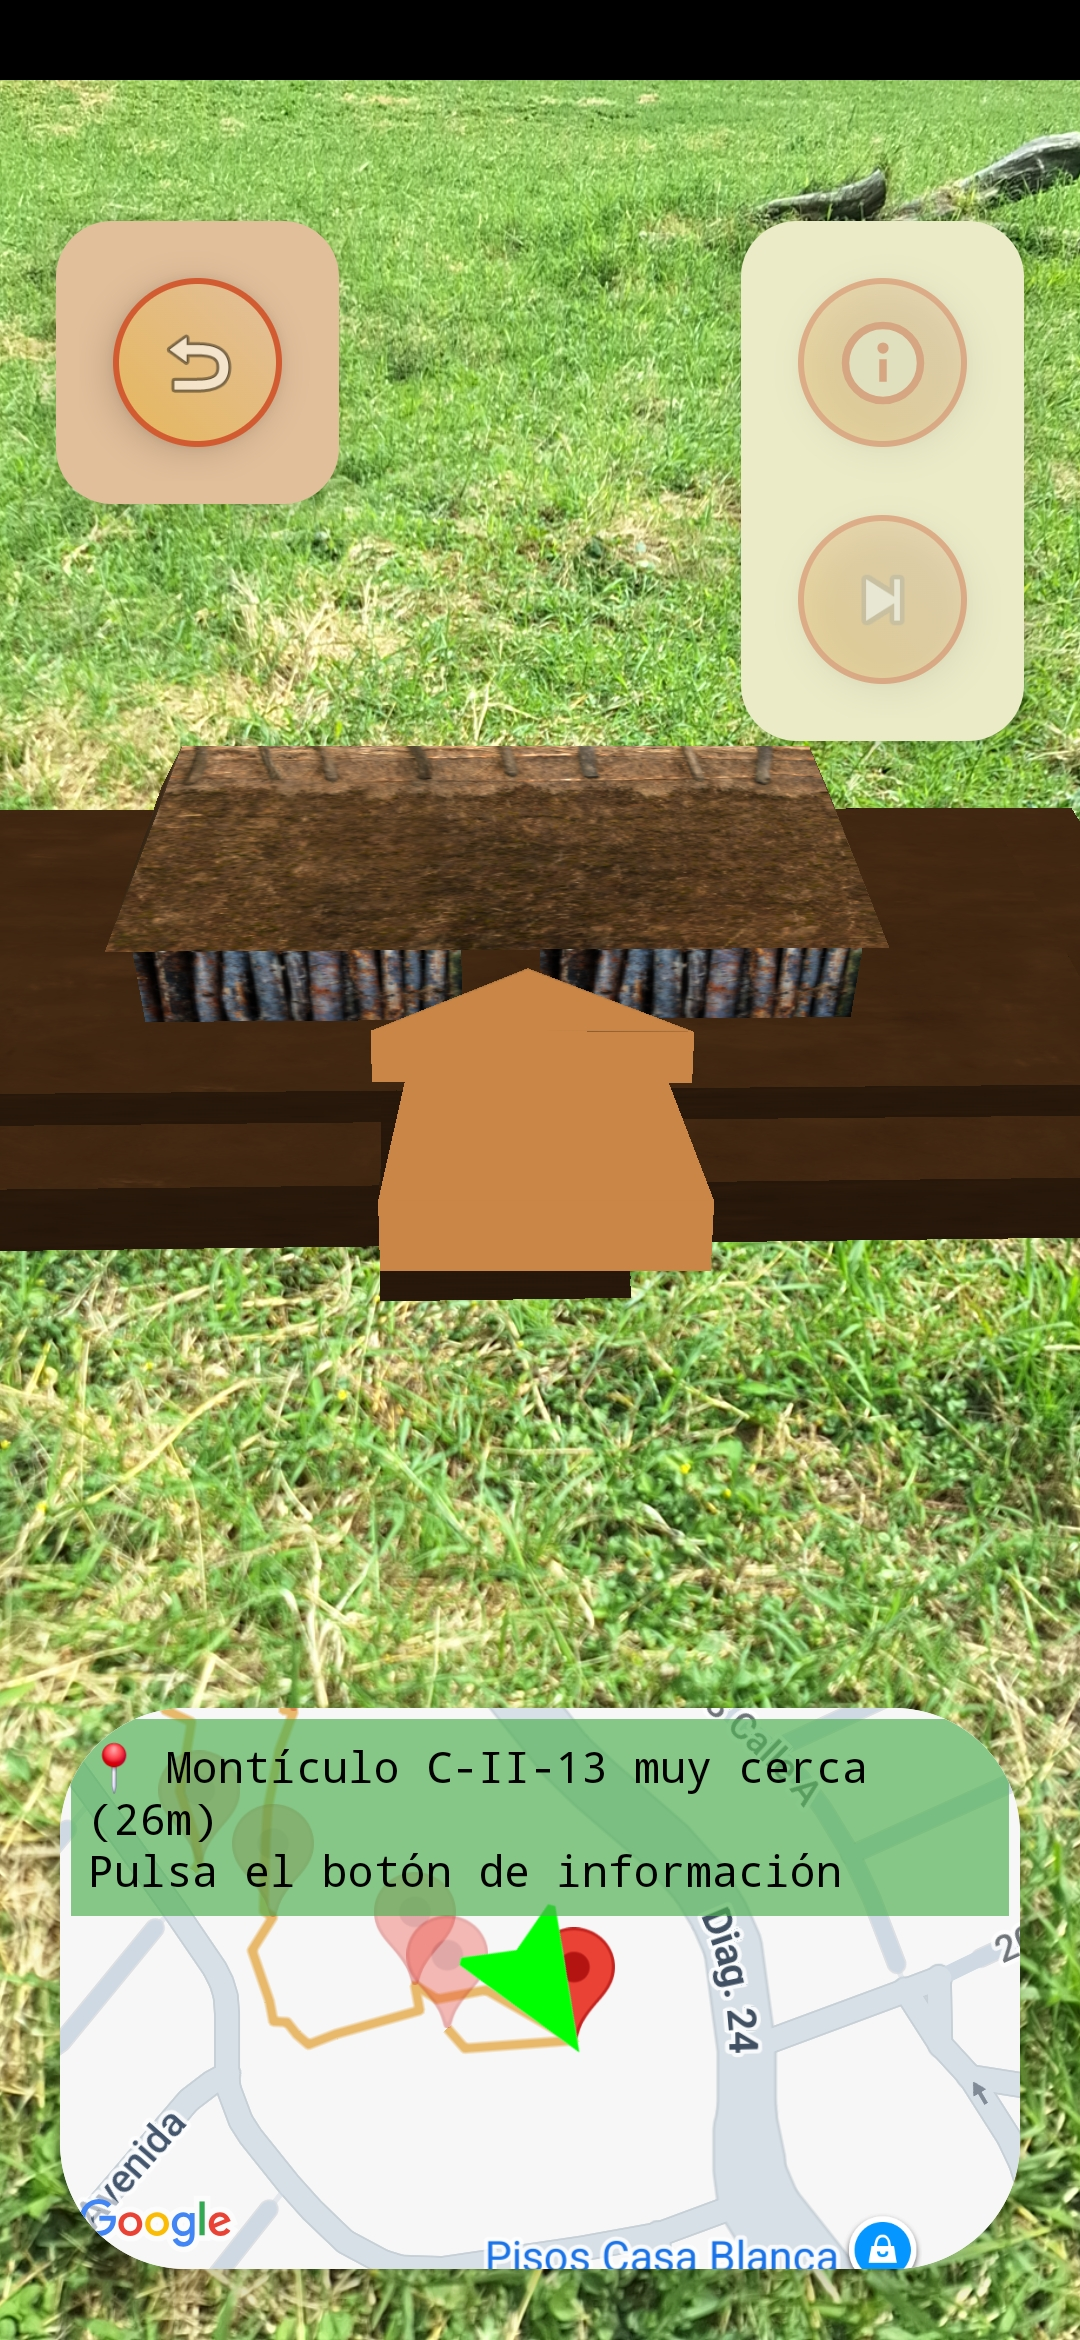
\includegraphics[width=0.28\linewidth]{resultados/figures/m13/m13_ar.jpg}
\end{figure}
\FloatBarrier
\clearpage
\FloatBarrier
\subsection{Montículo 14}

\begin{figure}[!htbp]
    \centering
    % ----- Fila 1 -----
    \begin{subfigure}{0.48\textwidth}
        \centering
        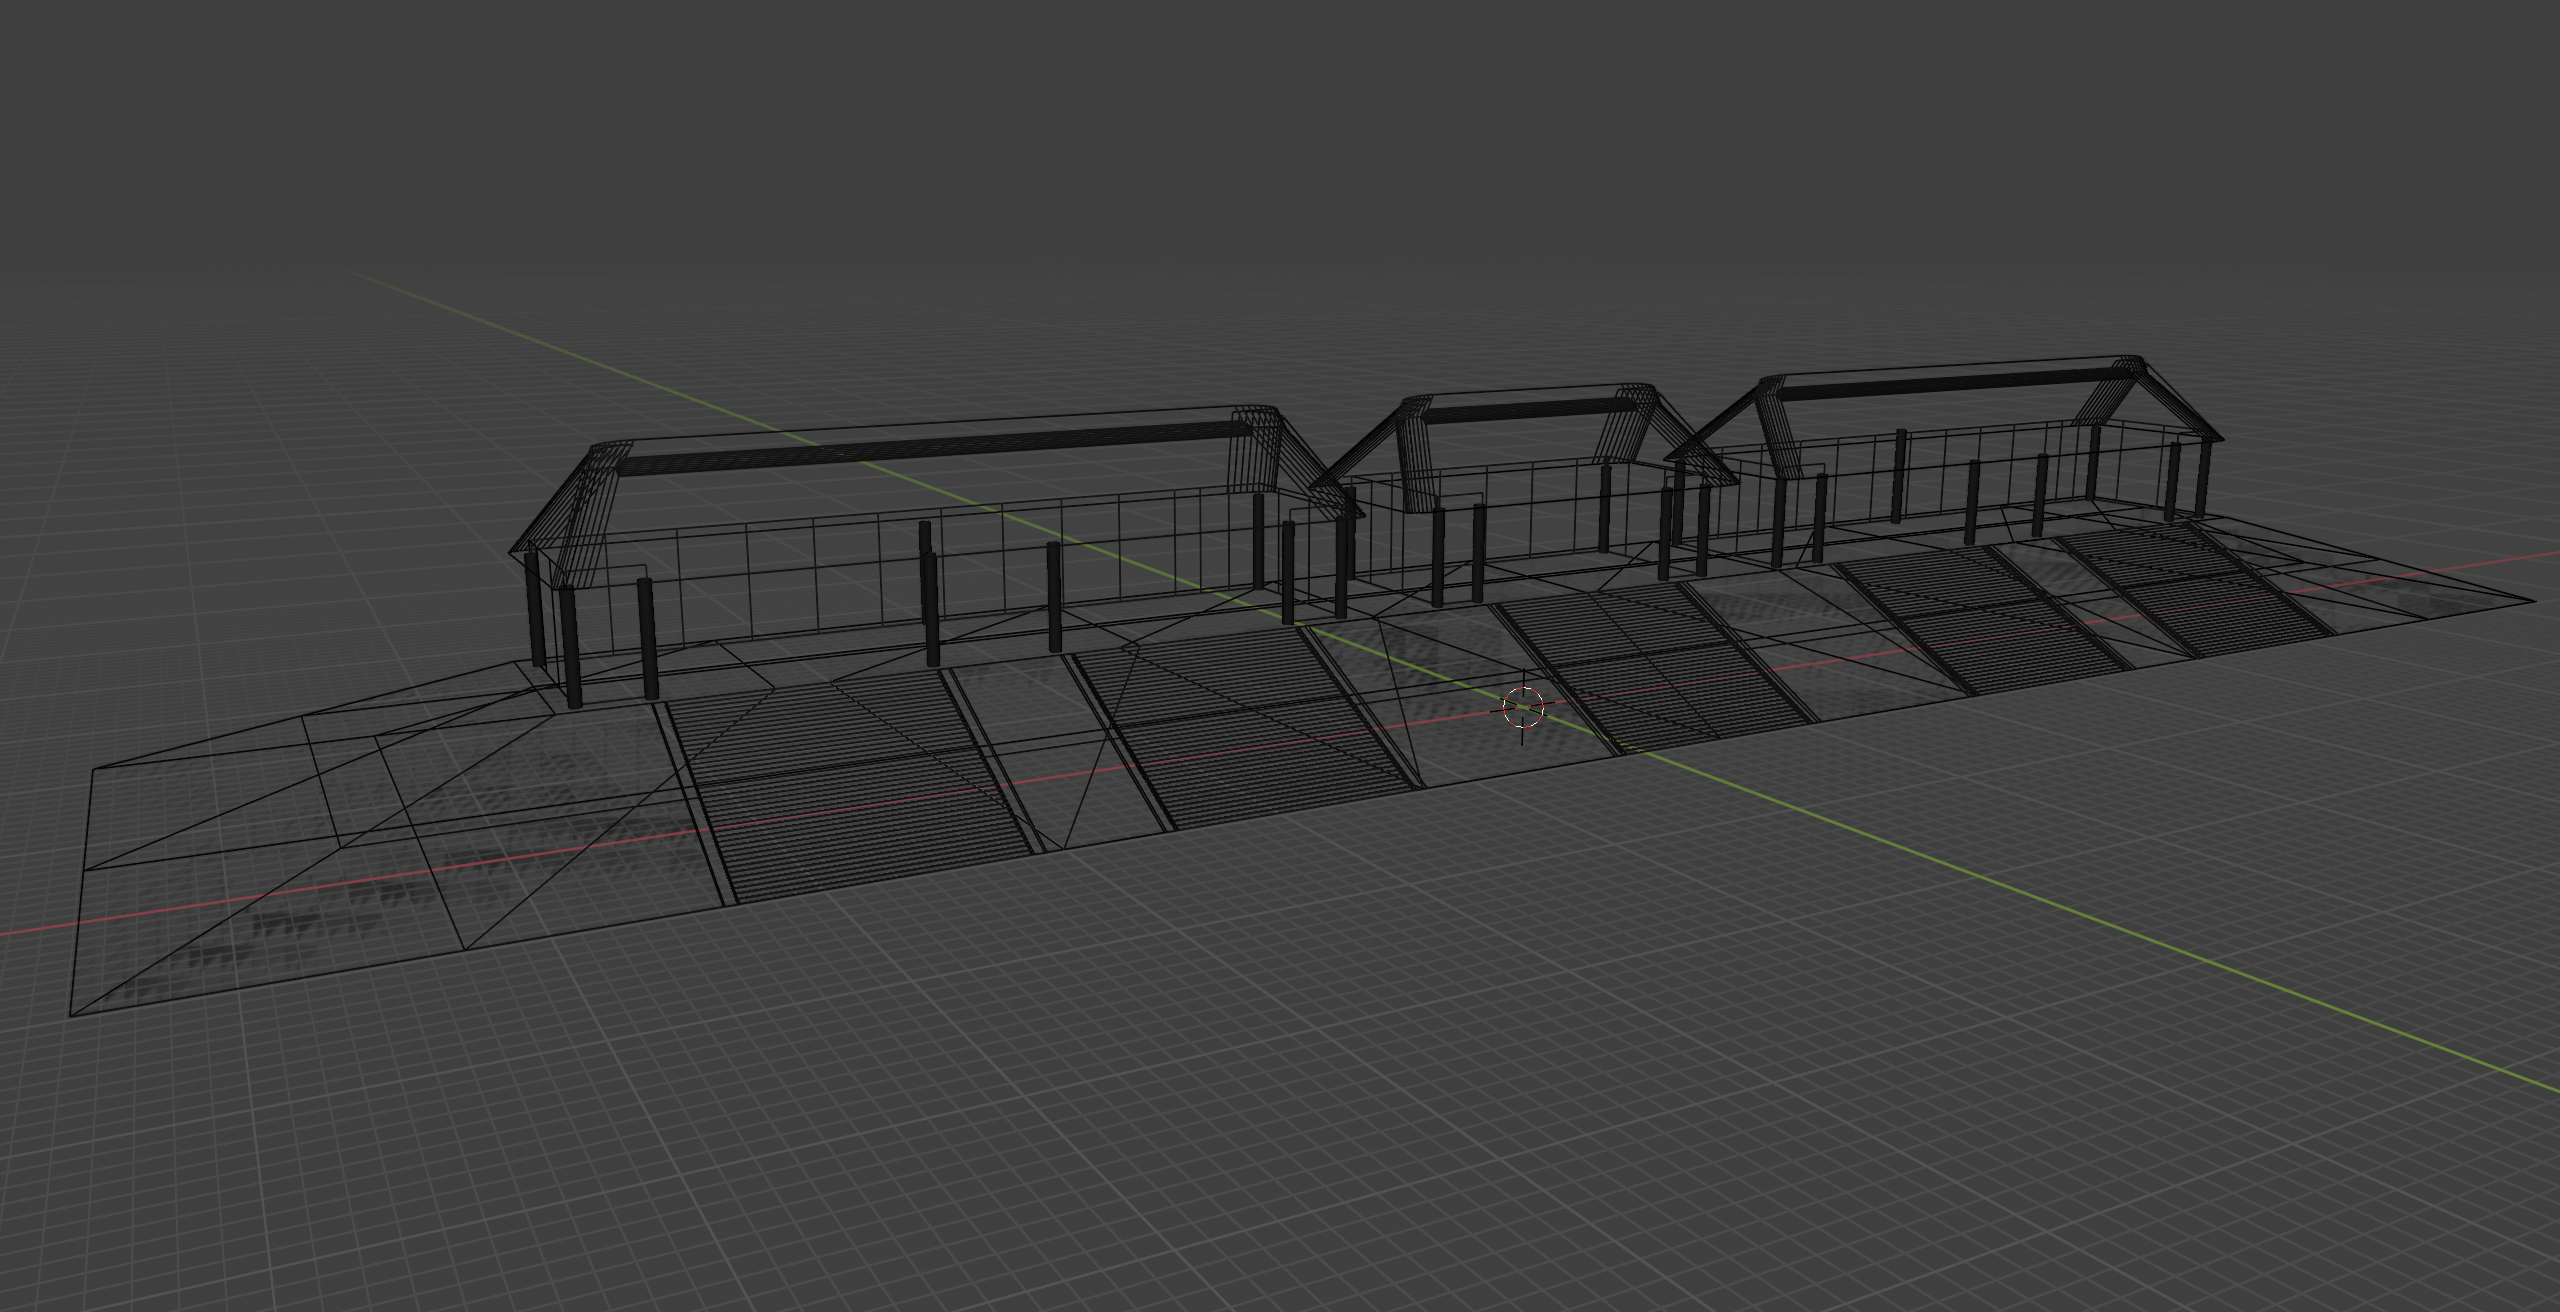
\includegraphics[width=0.85\linewidth]{resultados/figures/m14/m14_wireframe.png}
        \caption{Vista en malla (wireframe).}
        \label{fig:m14-wire}
    \end{subfigure}\hfill
    \begin{subfigure}{0.48\textwidth}
        \centering
        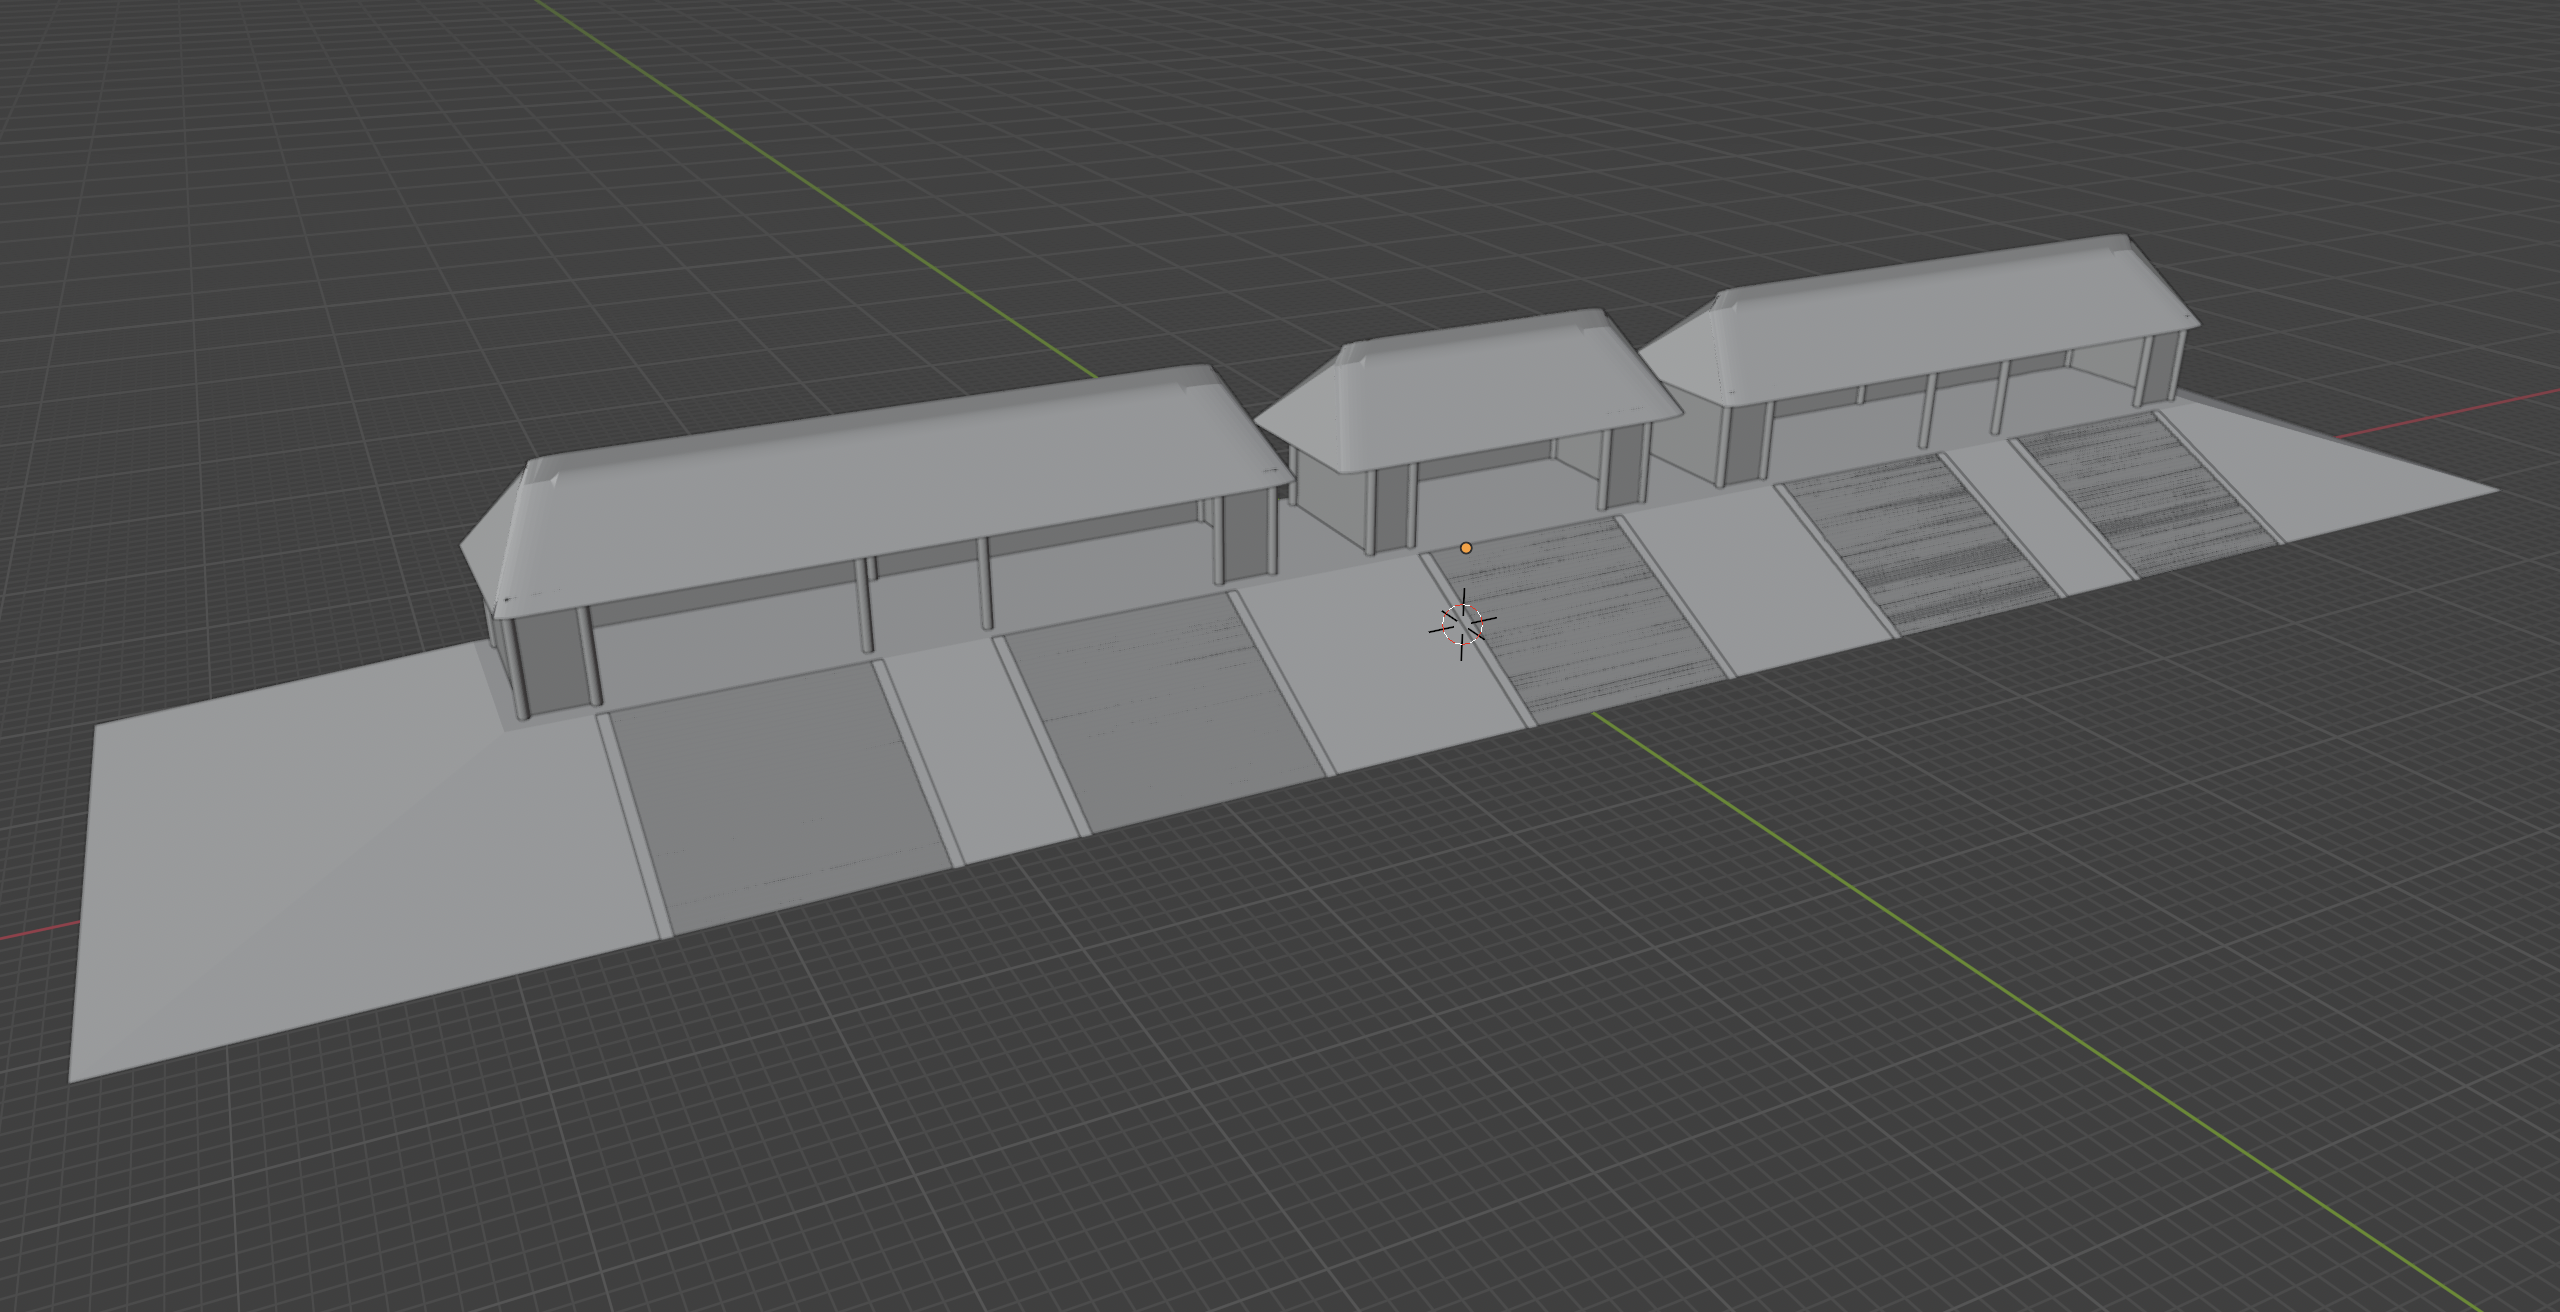
\includegraphics[width=0.85\linewidth]{resultados/figures/m14/m14_solid.png}
        \caption{Vista sólida sin texturas.}
        \label{fig:m14-solid}
    \end{subfigure}

    \vspace{0.5em}

    % ----- Fila 2 -----
    \begin{subfigure}{0.48\textwidth}
        \centering
        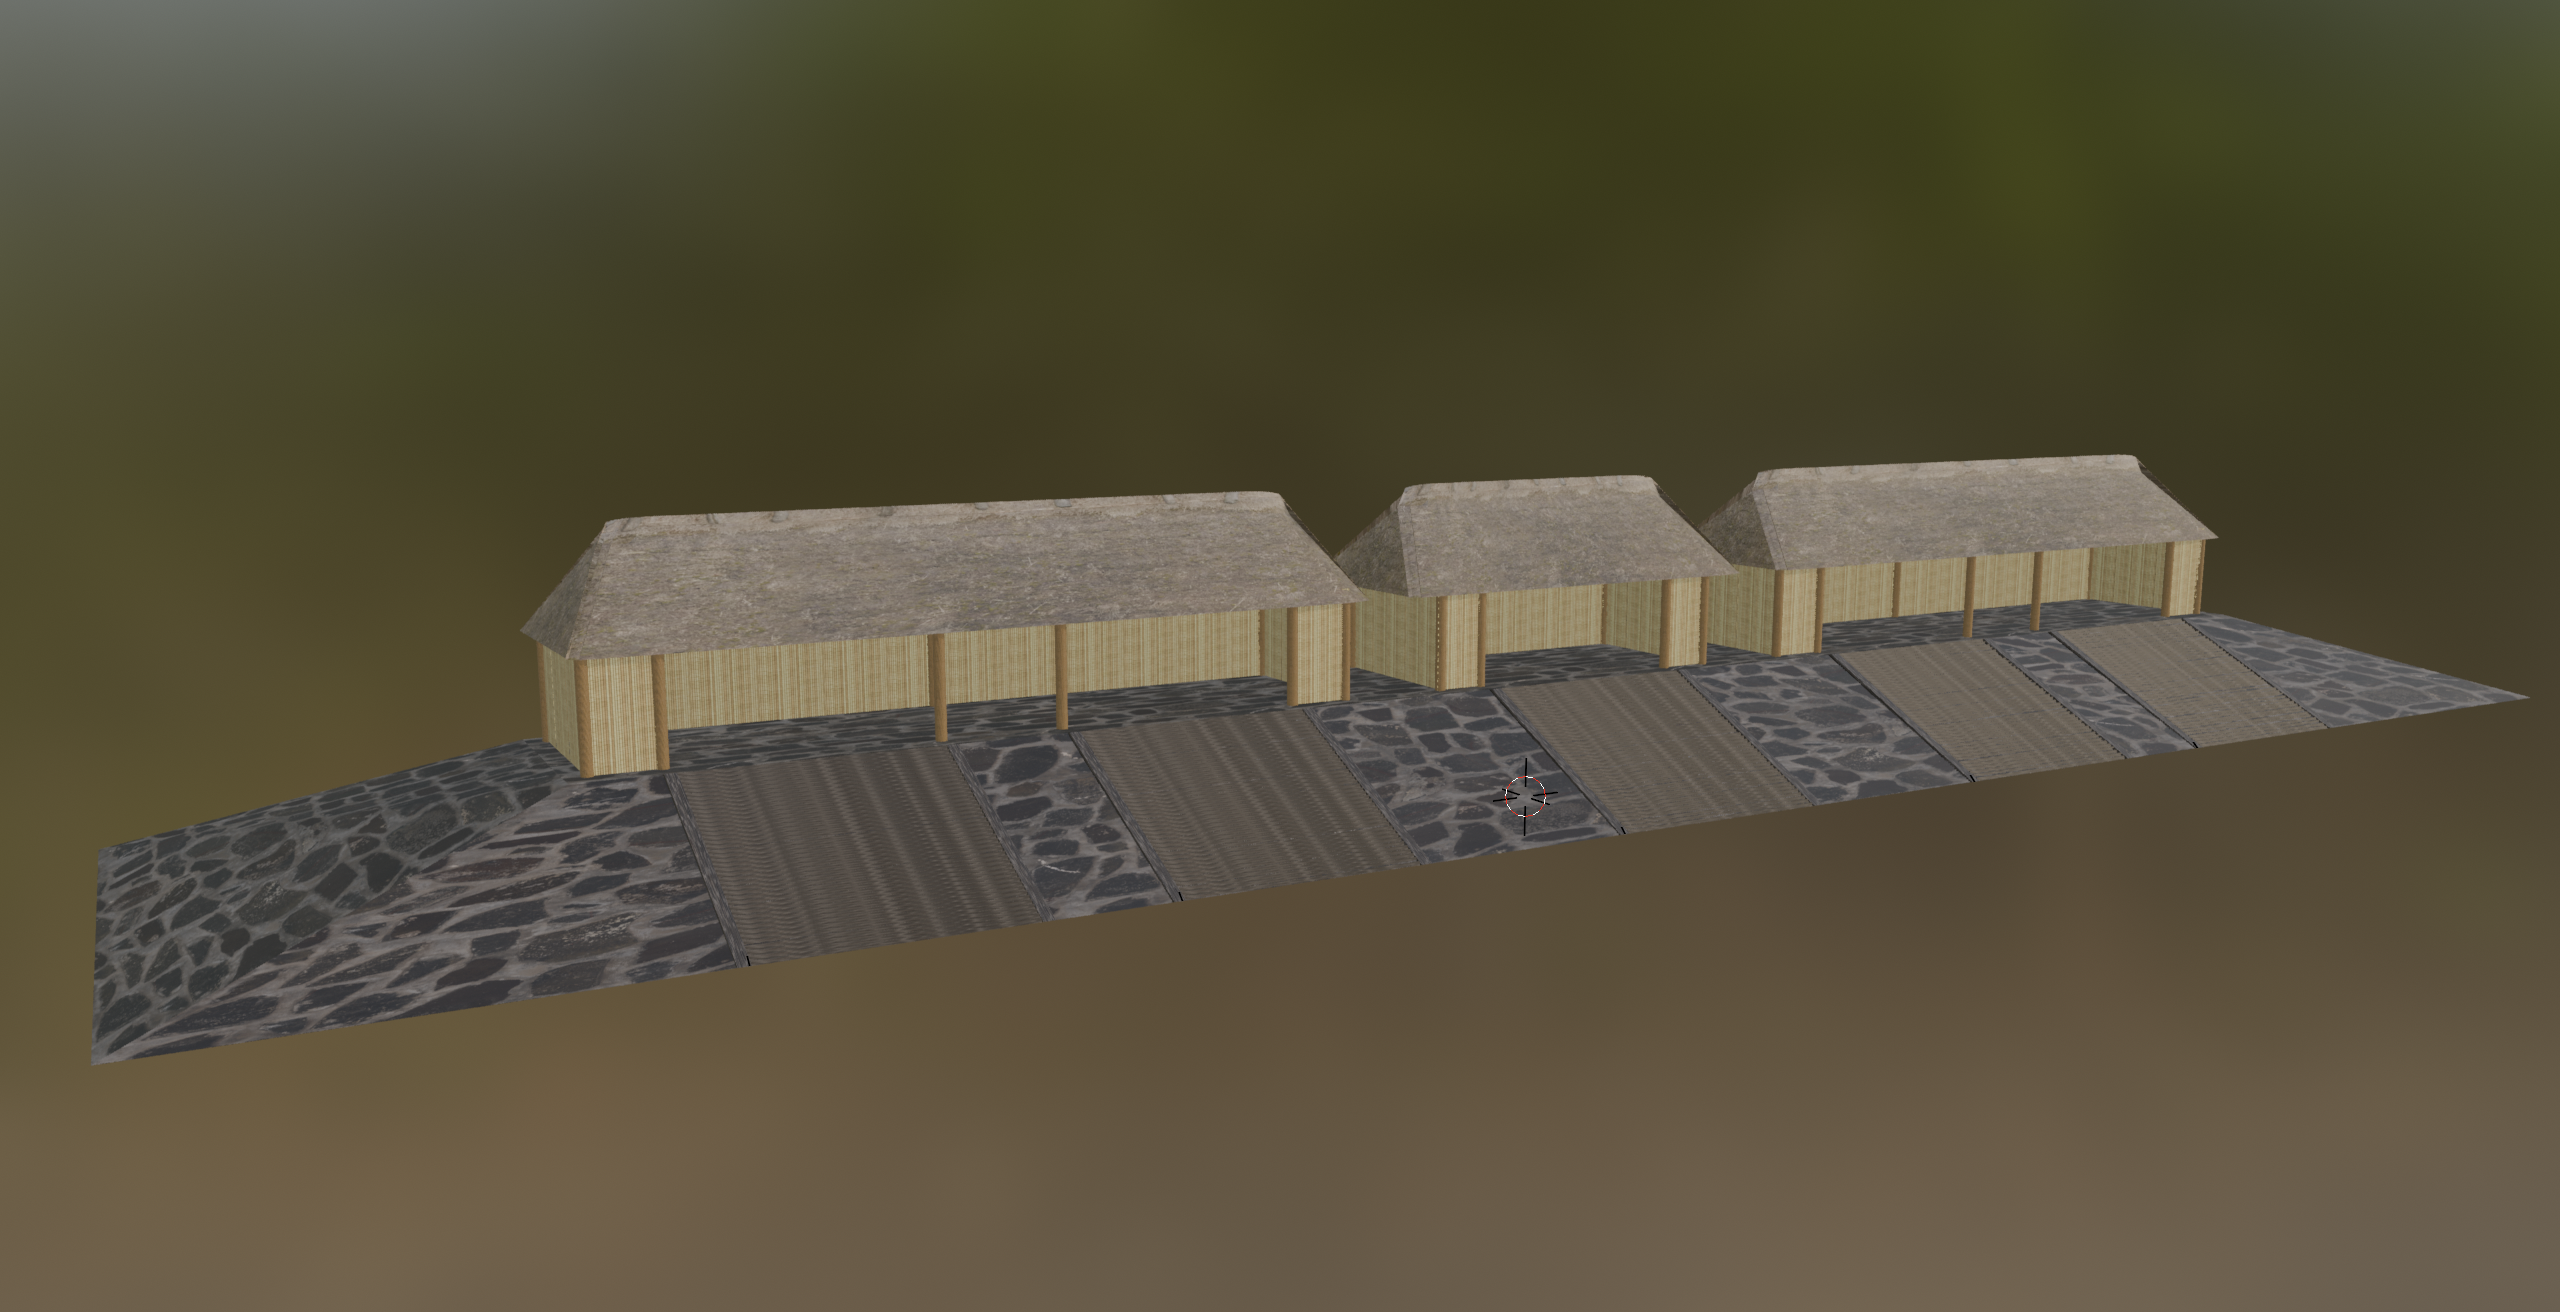
\includegraphics[width=0.85\linewidth]{resultados/figures/m14/m14_textured_viewport.png}
        \caption{Vista con materiales/texturas.}
        \label{fig:m14-textured}
    \end{subfigure}

    \caption{Montículo 14, panel de vistas.}
    \label{fig:m14-panel}
\end{figure}

\begin{figure}[!htbp]
    \centering
    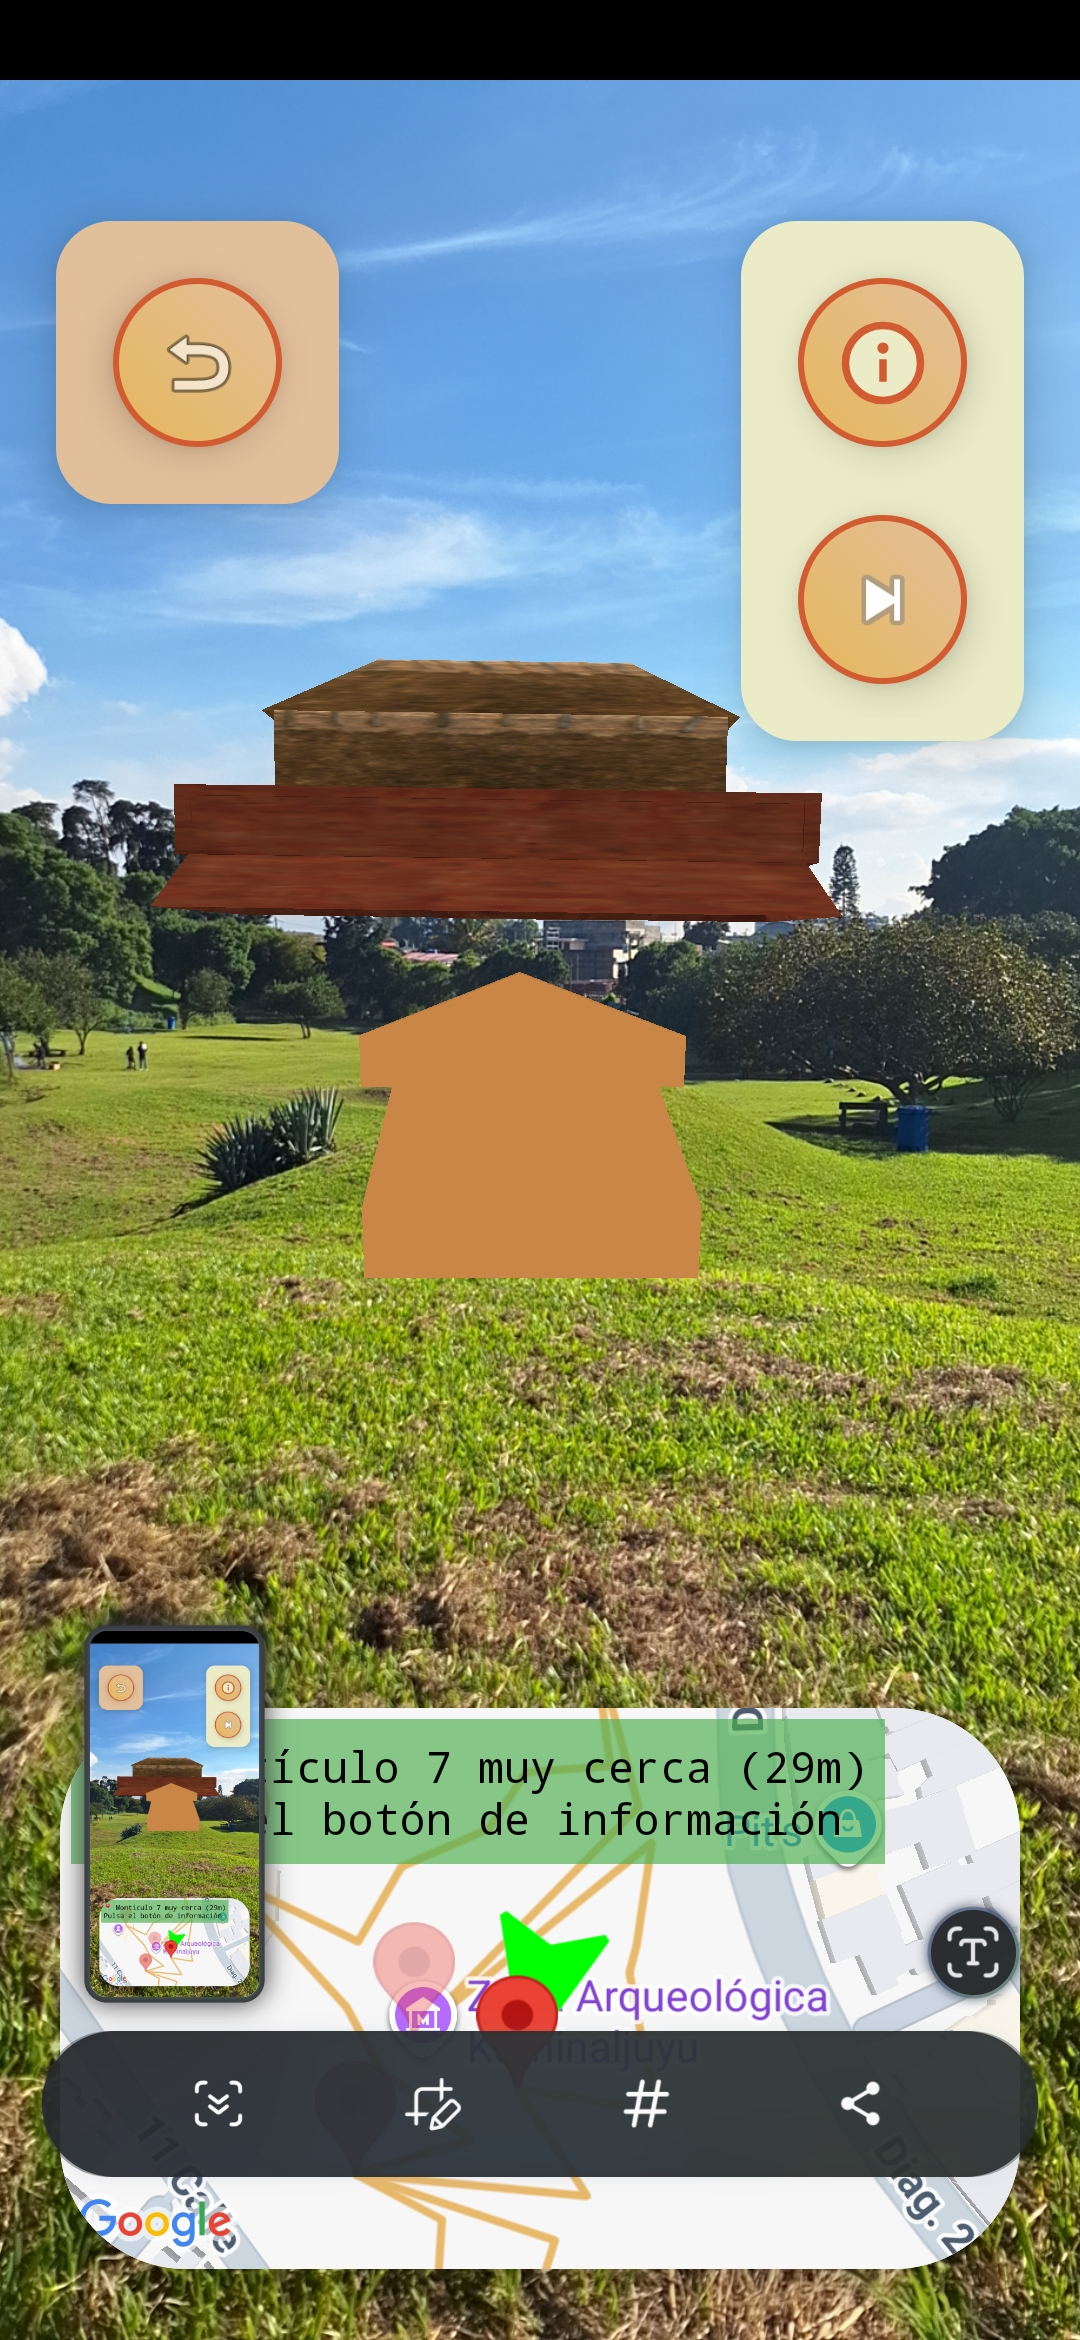
\includegraphics[width=0.28\linewidth]{resultados/figures/m3/m3_ar.jpg}
    \caption{Montículo 3 visualizado en la aplicación de realidad aumentada, mostrando la reconstrucción superpuesta en el entorno real del parque arqueológico.}
    \label{fig:m14-ar}
\end{figure}
\FloatBarrier
\clearpage
\subsection{Montículo La Palangana}
\FloatBarrier

\begin{figure}[H]
    \centering
    \caption{Montículo La Palangana, panel de vistas}
    \label{fig:palangana-panel}
    % ----- Fila 1 -----
    \begin{subfigure}{0.48\textwidth}
        \centering
        \caption{Vista en malla (wireframe)}
        \label{fig:palangana-wire}
        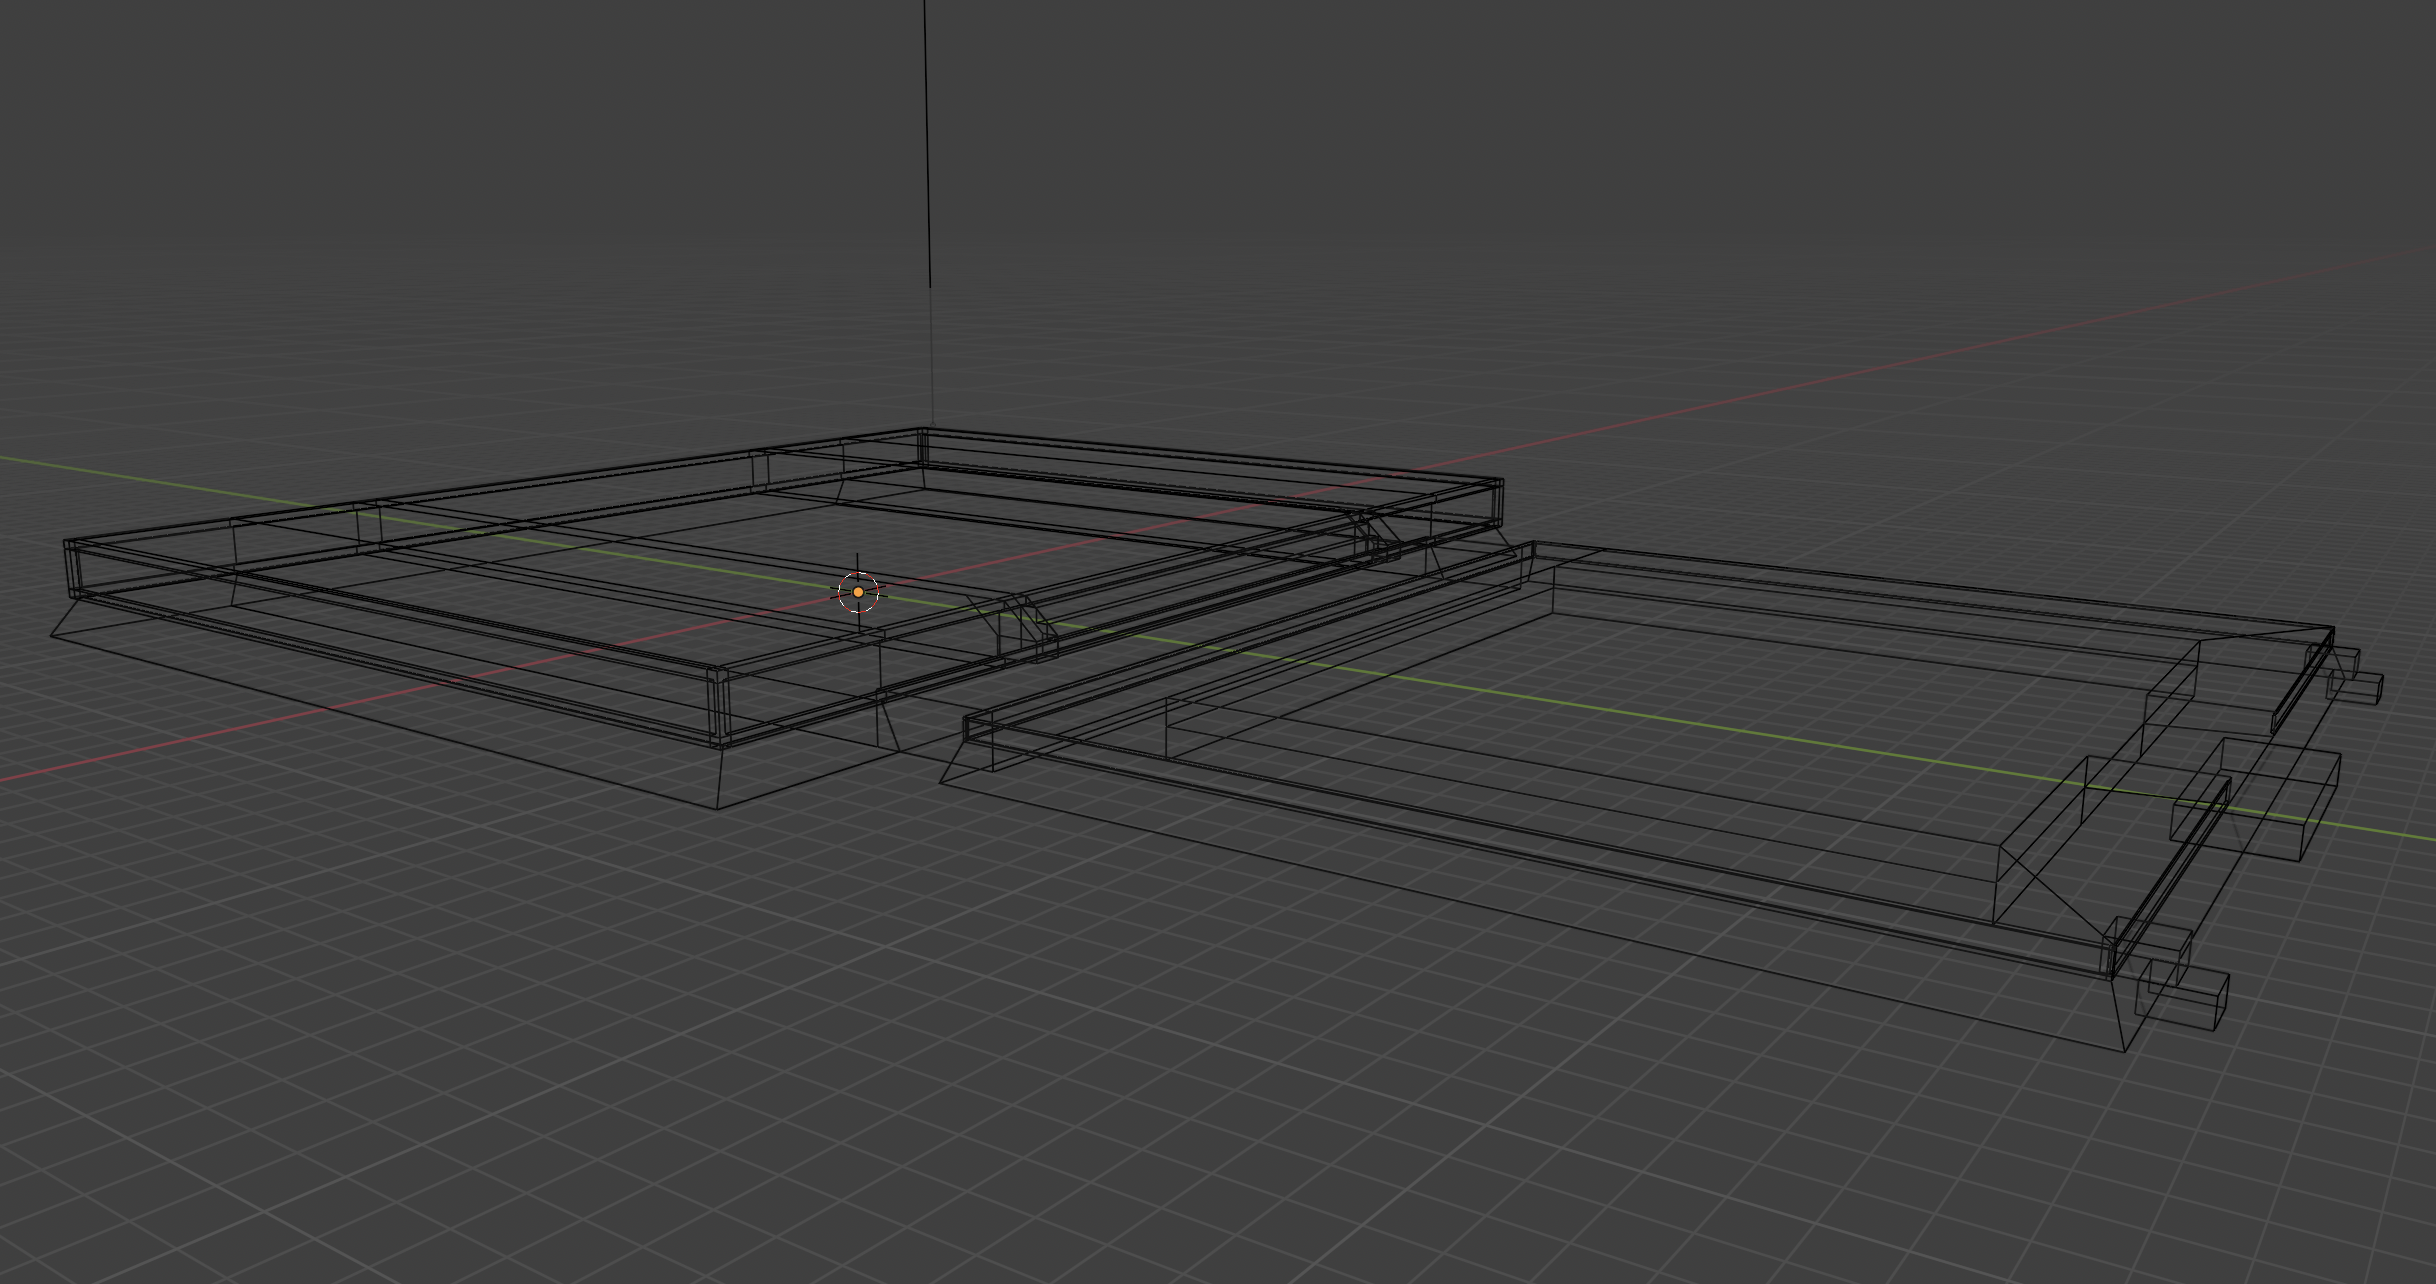
\includegraphics[width=0.85\linewidth]{resultados/figures/palangana/palangana_wireframe.png}
    \end{subfigure}\hfill
    \begin{subfigure}{0.48\textwidth}
        \centering
        \caption{Vista sólida sin texturas}
        \label{fig:palangana-solid}
        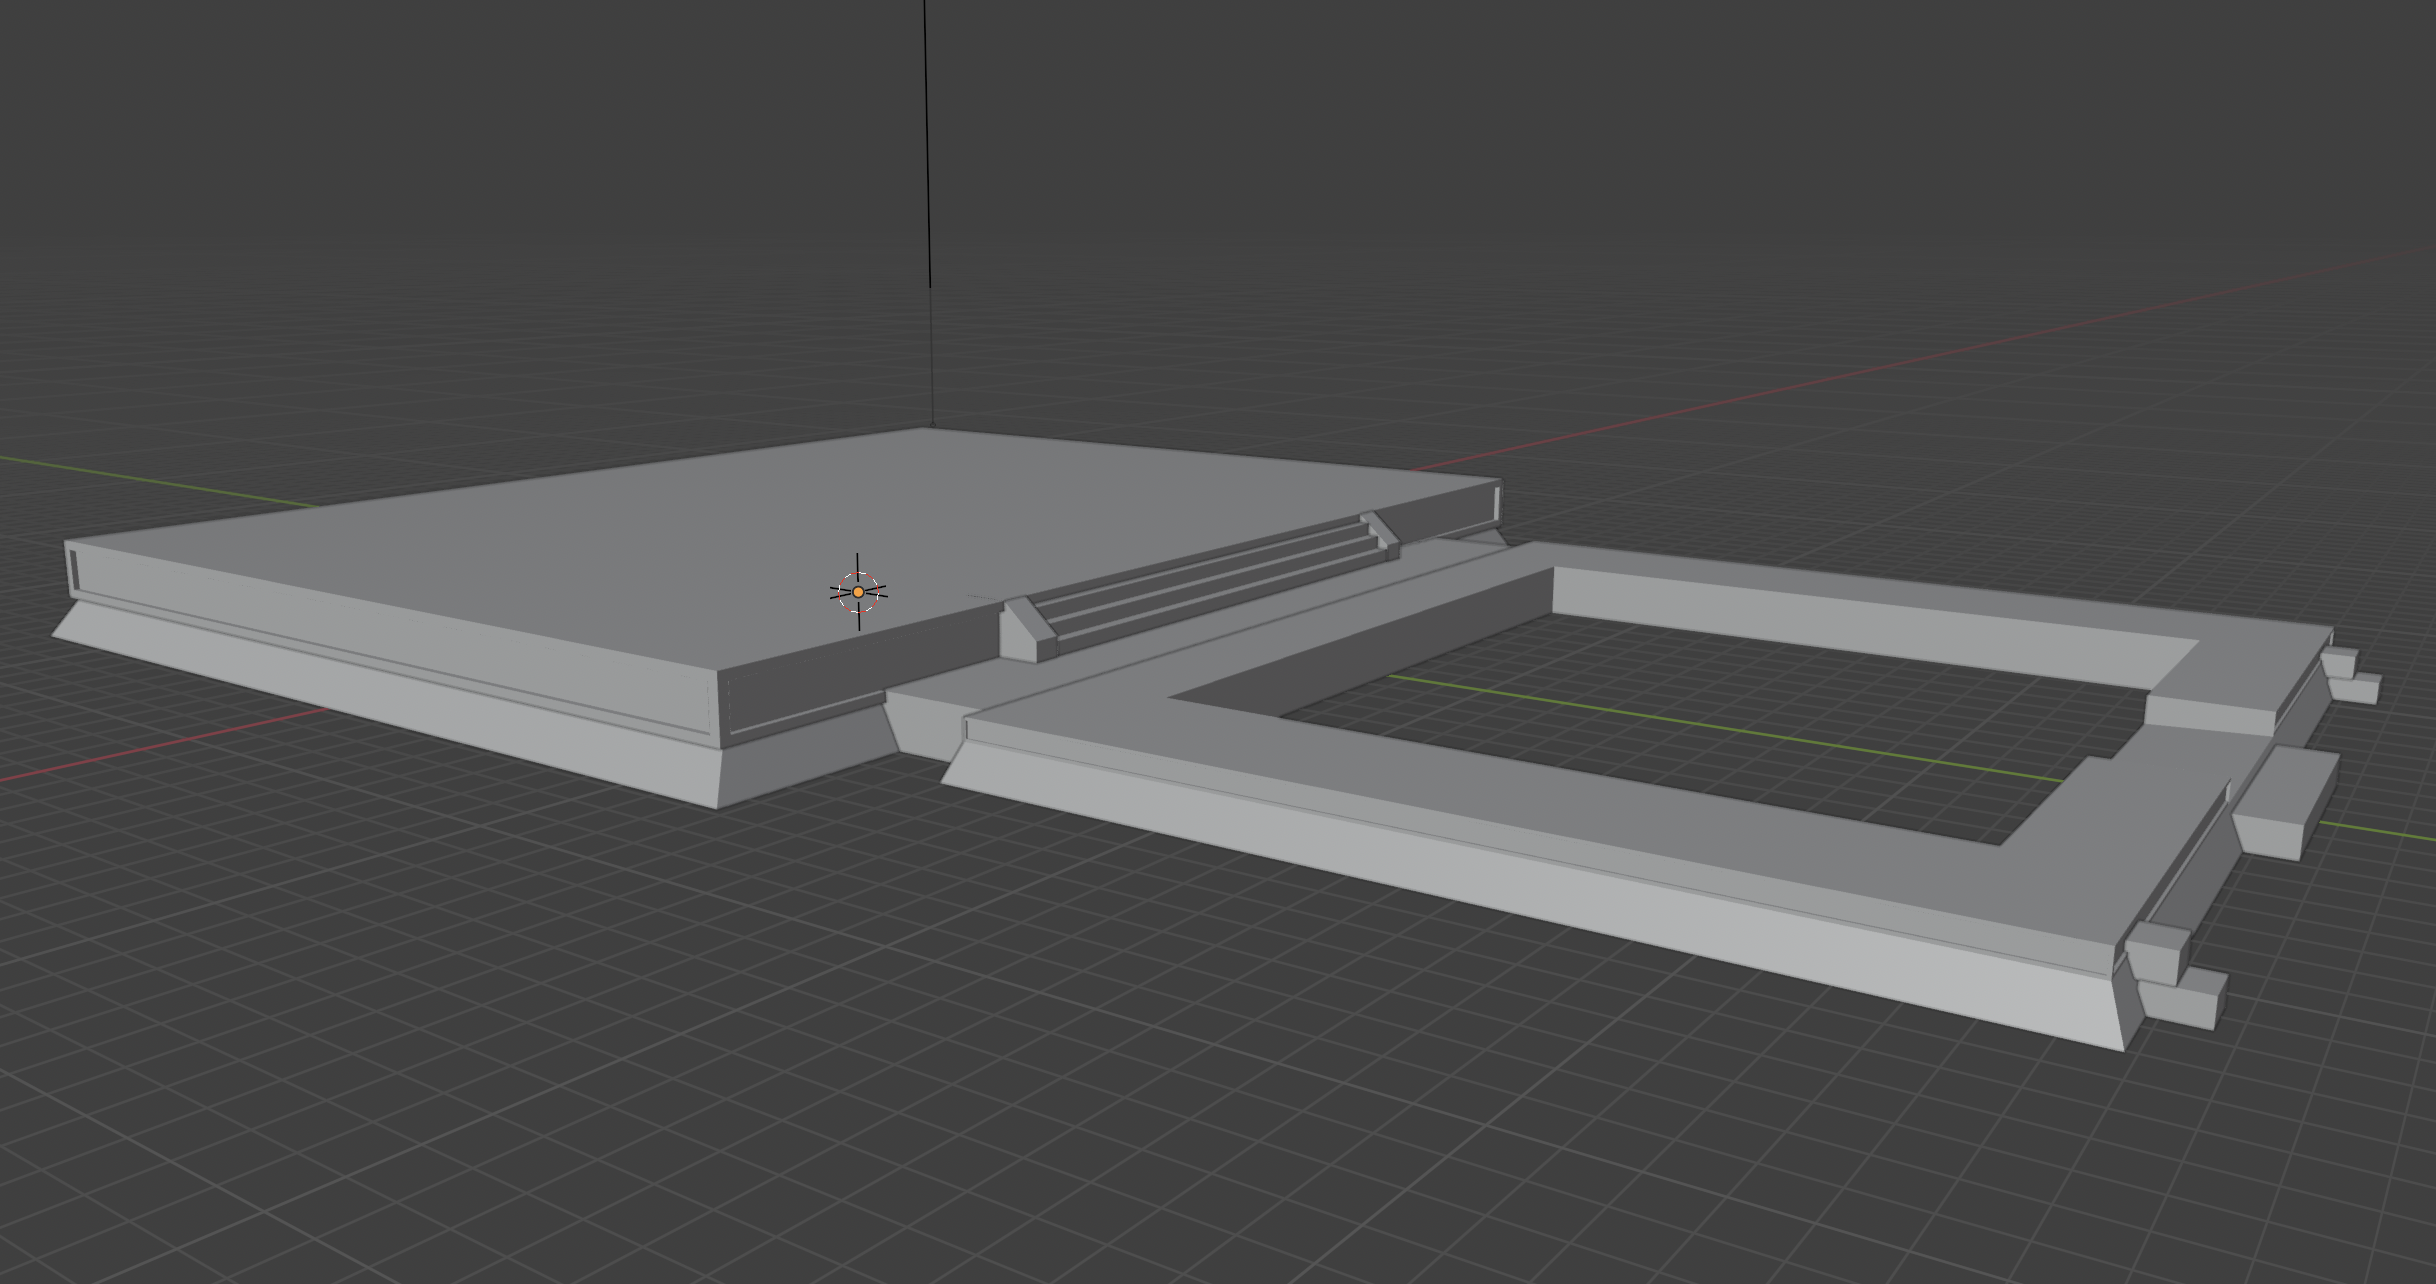
\includegraphics[width=0.85\linewidth]{resultados/figures/palangana/palangana_solid.png}
    \end{subfigure}

    \vspace{0.5em}

    % ----- Fila 2 -----
    \begin{subfigure}{0.48\textwidth}
        \centering
        \caption{Vista con materiales/texturas}
        \label{fig:palangana-textured}
        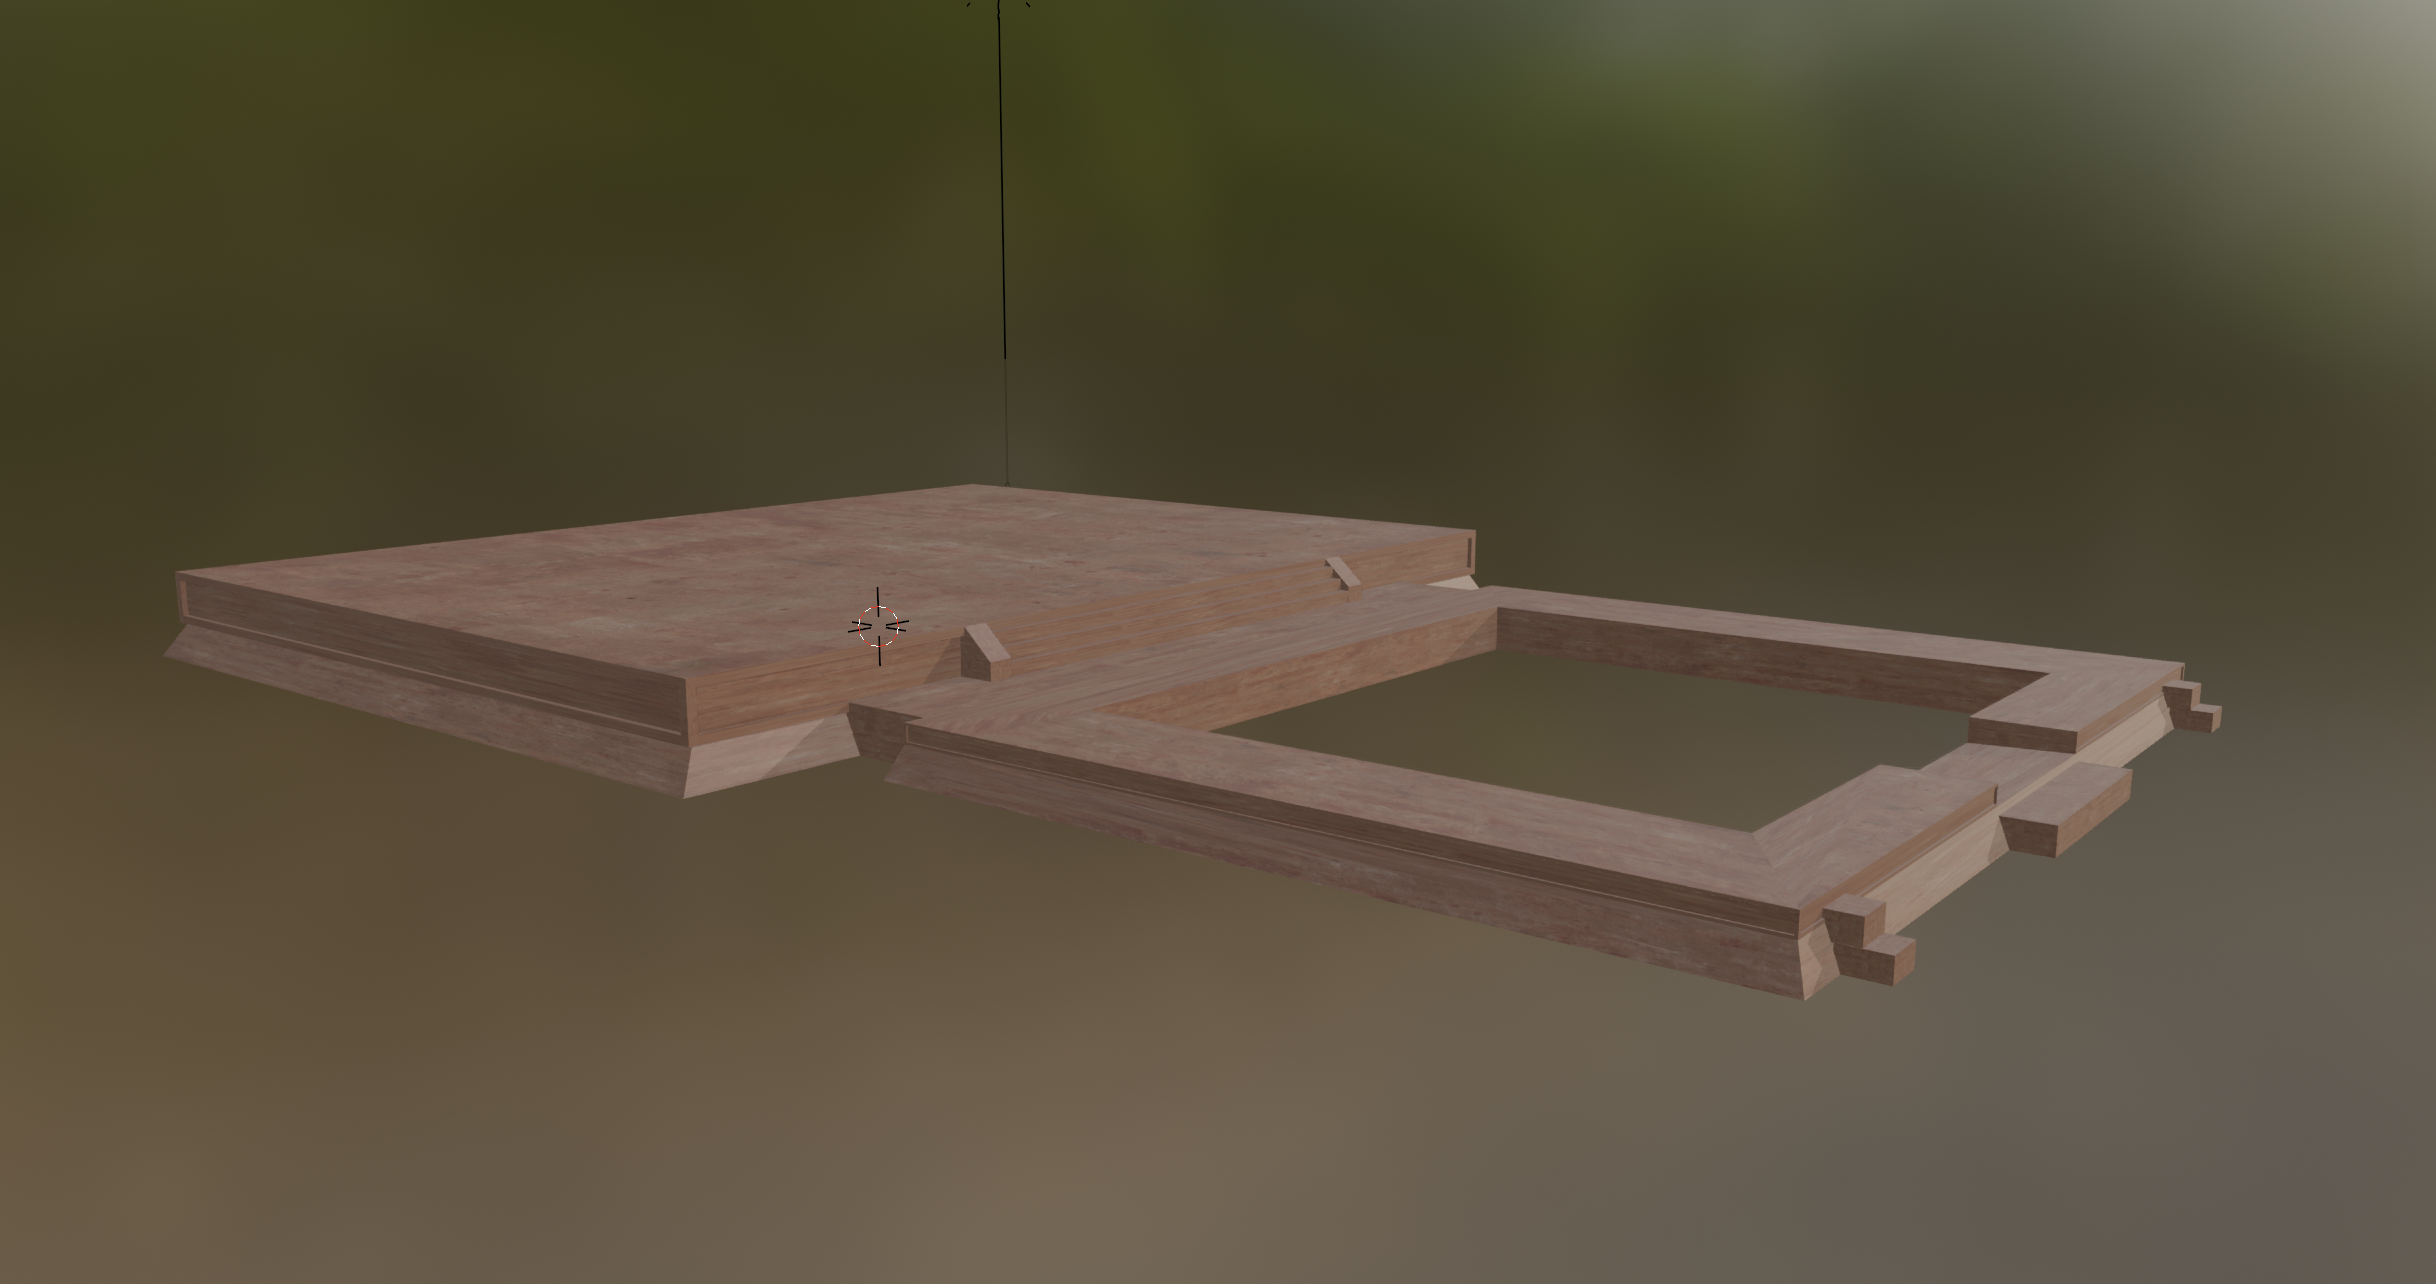
\includegraphics[width=0.85\linewidth]{resultados/figures/palangana/palangana_textured_viewport.png}
    \end{subfigure}
\end{figure}

\begin{figure}[!htbp]
    \centering
    \caption{Montículo La Palangana visualizado en la aplicación de realidad aumentada, mostrando la reconstrucción superpuesta en el entorno real del parque arqueológico}
    \label{fig:palangana-ar}
    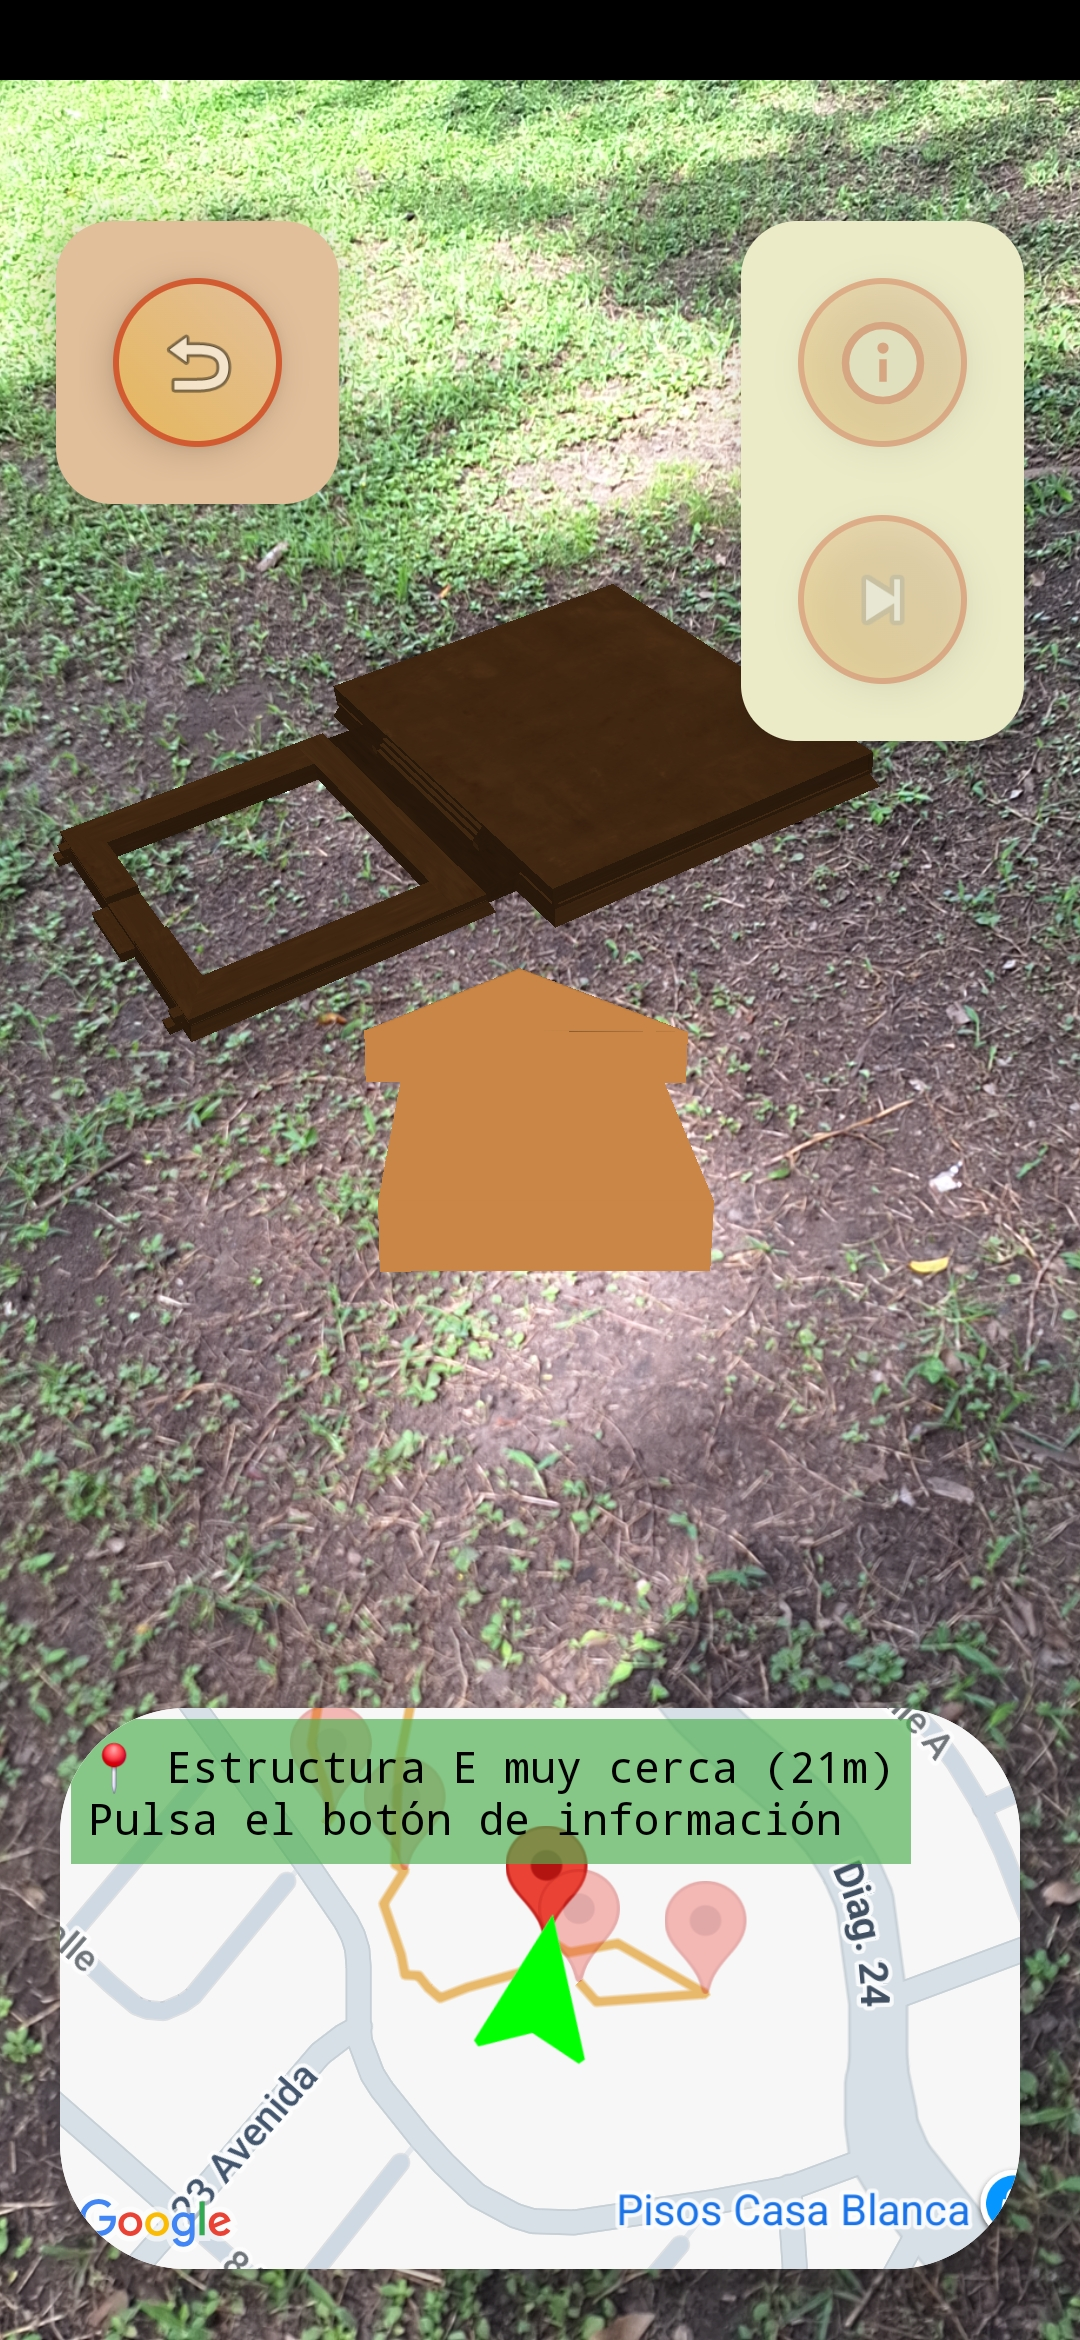
\includegraphics[width=0.28\linewidth]{resultados/figures/palangana/palangana_ar.jpg}
\end{figure}
\FloatBarrier
\clearpage

\subsection{Resultados de la encuesta}
\FloatBarrier

\begin{figure}[H]
    \centering
    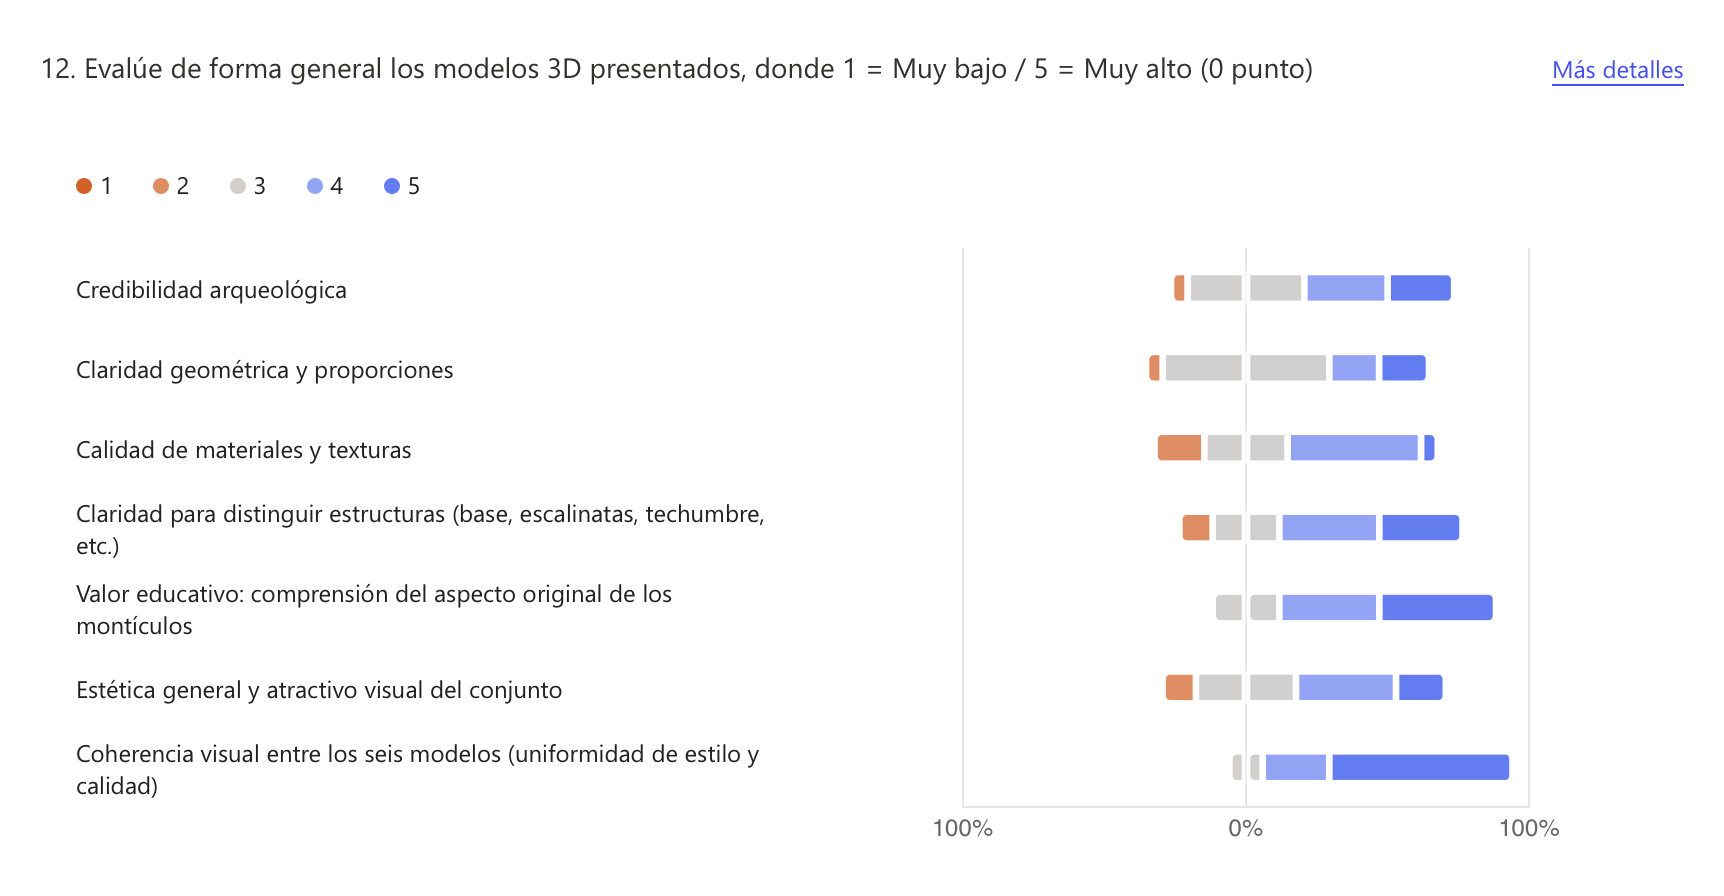
\includegraphics[width=\textwidth]{resultados/figures/Resultados_encuesta.png}
    \caption{Resultados de la encuesta aplicada a los usuarios.}
    \label{fig:resultados-encuesta}
\end{figure}

